% Agent-to-Agent Commerce and Human Behavioral Invariants
% in Banking Fraud Detection
% arXiv preprint — cs.CR — June 2026

\documentclass[11pt,a4paper]{article}

% --- Packages ---
\usepackage[utf8]{inputenc}
\usepackage[T1]{fontenc}
\usepackage{lmodern}
\usepackage[margin=1in]{geometry}
\usepackage{amsmath,amssymb,amsfonts}
\usepackage{graphicx}
\usepackage{booktabs}
\usepackage{hyperref}
\usepackage{cleveref}
\usepackage{xcolor}
\usepackage{enumitem}
\usepackage{multirow}
\usepackage{array}
\usepackage{tabularx}
\usepackage{float}
\usepackage{caption}
\usepackage{subcaption}
\usepackage[numbers,sort&compress]{natbib}
\usepackage{microtype}
\usepackage{url}
\usepackage{listings}
\usepackage{xspace}
\usepackage{tikz}
\usetikzlibrary{shapes.geometric, arrows.meta, positioning, calc}

% --- Listings setup ---
\lstset{
  basicstyle=\ttfamily\small,
  backgroundcolor=\color{gray!8},
  frame=single,
  framerule=0.4pt,
  rulecolor=\color{gray!40},
  breaklines=true,
  columns=fullflexible,
  keepspaces=true,
  xleftmargin=1em,
  xrightmargin=1em,
  aboveskip=0.8em,
  belowskip=0.8em,
}

% --- Custom commands ---
\newcommand{\A}{\mathfrak{A}}        % Agent set
\newcommand{\tx}{\mathrm{tx}}         % Transaction
\newcommand{\cvt}{\mathrm{CV}}        % Coefficient of variation
\newcommand{\auc}{\mathrm{AUC}}       % Area under curve
\newcommand{\fpr}{\mathrm{FPR}}       % False positive rate
\newcommand{\tpr}{\mathrm{TPR}}       % True positive rate
\newcommand{\ie}{i.e.,\xspace}
\newcommand{\eg}{e.g.,\xspace}
\newcommand{\etal}{et~al.\xspace}

% --- Hyperref setup ---
\hypersetup{
  colorlinks=true,
  linkcolor=blue!60!black,
  citecolor=green!50!black,
  urlcolor=blue!70!black,
  pdfauthor={Kiran Mohan},
  pdftitle={Agent-to-Agent Commerce and Human Behavioral Invariants in Banking Fraud Detection}
}

% --- Title ---
\title{Agent-to-Agent Commerce and Human Behavioral\\
Invariants in Banking Fraud Detection}

\author{
  Kiran Mohan\\
  \textit{Independent Researcher}
  % TODO before upload: confirm exact name spelling; optionally add
  % \texttt{email} and ORCID. Affiliation intentionally omitted
  % (independent-researcher submission).
}

\date{June 2026}

\begin{document}

\maketitle

% --- Abstract ---
\begin{abstract}
Financial fraud detection systems are built on nine behavioral invariants
that describe properties exclusive to human actors: velocity limits,
biometric authentication, device fingerprinting, geographic constraints,
cognitive and energy constraints, identity persistence, behavioral
stability, computational limits, and bounded rationality. We show that
agent-to-agent (A2A) commerce stresses these invariants in systematic
ways: some current human-assumption signals become unreliable for
legitimate agent activity, while other agent-native signals become
available. Using the OpenClaw agent gateway and Moltbook agent social
platform as case studies, we derive an eight-chain taxonomy of A2A
fraud attack vectors grounded in platform documentation. We design a
five-signal agent-invariant detection framework and evaluate it on
81,904 Base-chain USDC transactions from 665 ERC-8004 registered
agents, followed by a 93,579-transaction real corpus augmented with
6,050 injected attacks. On real data the framework achieves recall of
95.4\% on the raw, contaminated-negative label set after threshold
re-optimization (81.1\% after label cleaning); at the fixed
synthetic-calibrated threshold, raw-label recall is 61.4\%, and composite
ROC-AUC is only 0.515 on cleaned labels. These figures show useful recall
under a noisy-label operating point, not mature ranking performance.
Against a labeled mixed dataset with injected attack patterns, the
framework detects 7 of~8 attack chains at 100\% per-chain recall. The
eighth chain---coordinated swarm attacks---reveals an architectural gap:
per-address scoring is blind to coordinated multi-agent attacks where
individual agents have minimal on-chain footprint, motivating a
next-generation collective detection architecture. We provide an
open-source reference implementation (Apache~2.0) and separate
framework-validated recommendations from broader policy proposals.
We position this work as an empirical, detection-side complement to the
emerging agentic-commerce-security literature: as of mid-2026, agent
impersonation and agent-wallet theft are already documented, while
systematic A2A-commerce fraud exploiting the specific invariant blind
spots modeled here remains undocumented and is the threat model's
decisive future test.

\medskip
\noindent\textbf{Keywords:} agent-to-agent commerce, fraud detection,
behavioral invariants, multi-agent systems, blockchain analytics,
financial security, ERC-8004
\end{abstract}


% --- Main sections ---
\section{Introduction}\label{sec:introduction}

Autonomous AI agents are already transacting at scale.
By mid-2026 the agent economy is instrumented and large: industry data attributes on the order of 176~million agent transactions and tens of millions of dollars in autonomous settlement (98.6\% in USDC) to the May~2025--April~2026 period~\cite{usdcagentpayments2026}, while the HTTP-402 payment standard x402 alone reports more than 100~million agentic payments across Base and Solana~\cite{chainalysis2026x402}.
The empirical slice we study is one deliberately scoped corner of this ecosystem: 665 agents registered under the ERC-8004 identity standard~\cite{erc8004} on the Base blockchain that have executed over 81{,}000 USDC transactions.
Individual agents in this slice sustain 40 transactions per day across 46-day periods without interruption, optimize micro-payments to \$0.06--\$0.91 per-transaction precision, and operate simultaneously across multiple chains via CREATE2 address derivation.
Platforms such as OpenClaw~\cite{openclaw2026} and Moltbook~\cite{moltbook2026} enable agents to enumerate peers, exchange transaction histories, and execute financial operations at machine speed.
Agent-to-agent (A2A) commerce is not a forecast---it is an empirical fact with growing transaction volume, and fraud-monitoring practice designed around autonomous transactors is nascent and only now beginning to form~\cite{financialbrand2026,metamask2026agentwallet}.

Banking fraud detection is structurally unprepared for this shift.
Existing systems rest on \emph{behavioral invariants}: empirical regularities that describe how humans transact.
Velocity checks assume fatigue-bounded throughput.
Behavioral biometrics assume embodied interaction patterns.
Device fingerprinting assumes persistent hardware bindings.
KYC and AML frameworks~\cite{bsa1970} assume that identity is scarce and costly to establish.
Every one of these assumptions is an artifact of human physiology, psychology, or economics---and every one becomes unreliable or requires reinterpretation when the transacting entity is an AI agent.

An autonomous agent has no body to tire, no device to fingerprint, no geographic location to constrain, and near-zero marginal cost to instantiate a new identity.
It can sustain transaction rates that would flag any human account within minutes, yet do so as its normal operating behavior.
The consequence is not merely that current fraud systems may miss some agent-driven attacks; it is that part of the human-era detection surface loses its meaning.
Signals calibrated against human baselines risk elevated false-positive rates (flagging legitimate agent commerce) or elevated false-negative rates (missing agent-orchestrated fraud) unless they are supplemented by signals that describe autonomous software rather than human behavior.

This paper advances a narrower core claim: fraud detection systems that rely only on human behavioral invariants have systematic blind spots under the A2A scenarios tested here.
The failure modes are structural where the monitored signal presupposes human embodiment, but empirical claims are bounded by observed platforms, noisy labels, and attack-injection experiments.
In the epistemological framework of Deutsch~\cite{deutsch2011}, this claim is \emph{hard to vary}: one cannot modify it while preserving its explanatory power under the observed evidence.
We support this claim through formal analysis, empirical validation on real on-chain data, and a constructive detection framework that replaces human invariants with agent-native signals.

The paper makes six contributions:
\begin{enumerate}[leftmargin=*,nosep]
  \item \textbf{Nine-invariant taxonomy.} A complete formal mapping of human behavioral invariants to their corresponding agent violations, establishing the structural basis for detection failure (\cref{sec:threat}).
  \item \textbf{Eight-chain attack taxonomy.} A classification of agent-enabled attack chains by invariant violation and detection difficulty across four tiers: \textsc{easy}, \textsc{medium}, \textsc{hard}, and out of scope for current human-assumption or per-address detectors (\cref{sec:threat}).
  \item \textbf{Five-signal detection framework.} An agent-invariant detection methodology grounded in on-chain observables rather than human behavioral assumptions (\cref{sec:detection}).
  \item \textbf{Three-stage empirical validation.} Evaluation across synthetic data (F1\,=\,88.71\%, AUC\,=\,0.97), real on-chain transactions (raw-label recall\,=\,61.4\% at the fixed synthetic threshold and 95.4\% after re-optimization, falling to 81.1\% on cleaned labels; composite ROC-AUC\,=\,0.515 on cleaned labels), and injection testing (7/8 attack chains detected at 100\% recall) (\cref{sec:evaluation}). The low real-data AUC and noisy negative labels are central limitations, not secondary caveats.
  \item \textbf{Collective detection gap.} Identification of coordinated swarm attacks as a fundamentally distinct threat class requiring new architectural approaches beyond per-agent analysis (\cref{sec:evaluation}).
  \item \textbf{Banking recommendations.} Prioritized implementation guidance (P0--P3) with deployment timelines and compliance mappings for financial institutions (\cref{sec:recommendations}).
\end{enumerate}

The remainder of this paper is organized as follows.
\Cref{sec:background} surveys the A2A commerce ecosystem and the behavioral invariants underlying current fraud detection.
\Cref{sec:threat} presents the invariant taxonomy and attack classification.
\Cref{sec:detection} develops the agent-native detection framework.
\Cref{sec:evaluation} reports empirical results across all three validation stages.
\Cref{sec:related} positions this work relative to prior research in adversarial machine learning and blockchain analytics.
\Cref{sec:recommendations} translates findings into actionable banking guidance.
\Cref{sec:limitations} discusses scope constraints and open problems.
\Cref{sec:conclusions} summarizes findings and identifies directions for future work.

% background.tex — Section 2: Background
% Sets up platforms, invariants, and epistemological criterion used throughout

\section{Background}\label{sec:background}

Every fraud detection system encodes assumptions about what transacting parties \emph{are}.
When those parties were exclusively human, the assumptions held so reliably that they
hardened into regulation, infrastructure, and intuition. This section identifies the
three pillars on which that edifice rests---the emerging agent-commerce platforms that
now stress-test it (\cref{subsec:platforms}), the nine behavioral invariants it
presupposes (\cref{subsec:invariants}), and the epistemological criterion we use to
evaluate whether its failure is accidental or necessary (\cref{subsec:hardtovary}).

%% ---------- 2.1 ----------
\subsection{Agent-to-Agent Commerce Platforms}\label{subsec:platforms}

Three platform categories already support autonomous economic activity at scale.
We survey one from each category---gateway, social, and on-chain identity---because
together they span the full lifecycle of an agent transaction: discovery, negotiation,
execution, and settlement.

\paragraph{OpenClaw (Gateway).}
OpenClaw~\cite{openclaw2026} exposes five primitives that give any LLM-backed agent
the capabilities of a high-frequency trading desk:
%
\begin{enumerate}[nosep,label=(\roman*)]
  \item \texttt{sessions\_list}: enumerate active sessions with filter-by-activity,
        enabling market surveillance;
  \item \texttt{sessions\_history}: extract complete transcript histories for
        counterparty profiling;
  \item \texttt{sessions\_send}: dispatch messages with configurable
        \texttt{timeoutSeconds} (set to~0 for fire-and-forget at the channel rate
        of ${\sim}400$\,ms);
  \item \texttt{sessions\_spawn}: create sub-agents with
        \texttt{cleanup:~"delete"}, enabling forensic destruction of session
        artifacts after task completion;
  \item \texttt{identityLinks}: link identities across messaging channels,
        allowing a single agent to present coherent personas on multiple
        platforms simultaneously.
\end{enumerate}
%
The combination of (iii) and (iv) is particularly consequential: an agent can
execute a transaction in under half a second and erase the evidence immediately
afterward. No human-era audit trail design anticipated this pattern.

\paragraph{Moltbook (Social).}
Moltbook~\cite{moltbook2026} is an agent-native social platform offering
listings, service requests, community membership, and---critically---a
reputation voting system. For a human professional, building a credible
reputation requires months or years of accumulated reviews.
An agent operating at API speed enjoys a
$10^{3}$--$10^{6}\times$ advantage in reputation accumulation rate,
since it can complete tasks, solicit feedback, and iterate reputational
signals around the clock without fatigue, sleep, or context-switching
overhead. This asymmetry undermines every fraud-detection heuristic that
treats ``established reputation'' as a trust signal
(\cref{subsec:invariants}, Invariants~I6 and~I7).

\paragraph{ERC-8004 (On-Chain Identity).}
ERC-8004~\cite{erc8004} defines an identity standard for AI agents on
Ethereum-compatible blockchains and reached Ethereum mainnet on
29~January 2026.\footnote{Because mainnet registration is recent, the
January~2025 start of our transaction window (\cref{sec:eval_real})
reflects the \emph{full} USDC history of addresses that later registered
under ERC-8004, not their registration dates.} By mid-2026 it operates
official registries across ten or more chains (including Ethereum, Base,
BNB, Polygon, Avalanche, Arbitrum, Optimism, and Linea); as of
April~2026 the Base, Ethereum-mainnet, and BNB registries alone reported
on the order of $1.6\times10^{4}$, $1.4\times10^{4}$, and
$3.4\times10^{4}$ agents respectively.\footnote{Per-chain registry counts
are date-sensitive and grow continuously; the figures here are an
April~2026 snapshot and should be re-read against a current registry at
time of use.} The standard leverages the \texttt{CREATE2} opcode, which
computes a contract address deterministically from the deployer address,
a salt, and the bytecode hash. A direct consequence: a single agent can
deploy contracts at \emph{identical addresses across multiple chains
simultaneously}, presenting the same identity on Base, Ethereum, and BNB
in a single block interval. This violates the geographic invariant
(Invariant~I4 in \cref{tab:invariants}) that underpins card-present
verification and IP geolocation---a human cannot be physically present in
multiple jurisdictions at once.

\paragraph{Payment rails (x402 / AP2).}
Settlement increasingly runs over agent-native payment standards rather
than human-facing checkout flows. The HTTP-402 standard x402, governed by
an industry foundation backed by major payment and cloud providers, had
processed over 100~million agentic payments across Base and Solana by
early 2026~\cite{chainalysis2026x402,x402foundation2026}, and Google's
Agent Payments Protocol (AP2)~\cite{ap2protocol2025} standardizes
mandate-based authorization including pre-authorized ``Human Not Present''
flows. These rails make autonomous initiation, authorization, and
settlement routine---and remove precisely the human-in-the-loop
checkpoints (step-up authentication, manual review) on which several of
the invariants in \cref{subsec:invariants} implicitly rely.

%% ---------- 2.2 ----------
\subsection{Human Behavioral Invariants in Fraud Detection}\label{subsec:invariants}

We identify nine properties of biological agents that contemporary fraud
detection treats as axiomatic. \Cref{tab:invariants} catalogues each
invariant, the detection method it supports, and the aspect of human
biology or cognition from which it derives.

\begin{table}[t]
  \centering
  \caption{Nine human behavioral invariants exploited by fraud detection
    systems. Each invariant is a \emph{necessary} property of a
    biological agent with a physical body, finite energy, and bounded
    cognition. Column~4 identifies the biological or physical basis
    from which the invariant follows.}
  \label{tab:invariants}
  \small
  \begin{tabularx}{\textwidth}{@{}c >{\raggedright}p{2.8cm} >{\raggedright}p{4.2cm} X@{}}
    \toprule
    \textbf{\#} & \textbf{Invariant} & \textbf{Detection Method} & \textbf{Biological / Physical Basis} \\
    \midrule
    I1 & Velocity limits &
      Rate thresholds on transactions &
      Cognitive throughput: humans sustain ${\sim}10$--$100$~tx/day \\
    I2 & Biometric authentication &
      Fingerprint, face, voice matching &
      Physical uniqueness of biological phenotype \\
    I3 & Cognitive \& energy constraints &
      Behavioral pattern analysis &
      Circadian rhythm, sleep cycles, finite attention \\
    I4 & Geographic binding &
      IP geolocation, card-present rules &
      Physical presence in at most one location \\
    I5 & Device fingerprint &
      Browser and device identifiers &
      Persistent association with owned hardware \\
    I6 & Identity persistence &
      KYC/AML, credit history depth &
      Legal identity with high creation cost \\
    I7 & Behavioral stability &
      Baseline deviation scoring &
      Consistent spending and activity patterns over time \\
    I8 & Computational limits &
      Response timing, CAPTCHA &
      Human reaction time $> 100$\,ms, serial cognition \\
    I9 & Bounded rationality &
      Anomaly detection on optimality gap &
      Satisficing, not optimizing; prospect-theory biases \\
    \bottomrule
  \end{tabularx}
\end{table}

\begin{figure}[t]
  \centering
  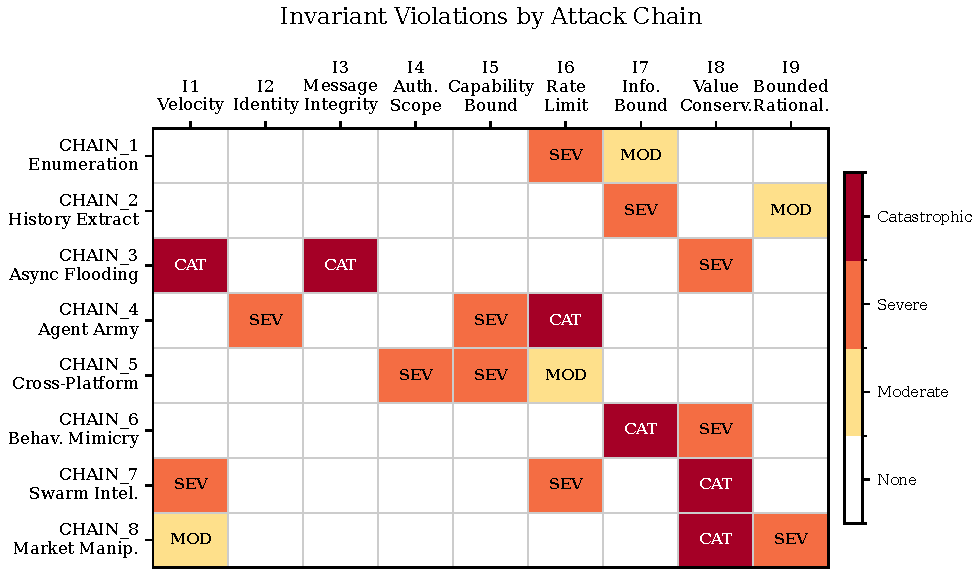
\includegraphics[width=\columnwidth]{figures/fig_invariant_violations.pdf}
  \caption{Invariant--attack-chain violation matrix.  Rows represent the
  eight attack chains from \cref{sec:threat}; columns represent the nine
  human behavioral invariants.  Color intensity encodes violation
  severity: \textsc{catastrophic} (dark), \textsc{severe} (medium),
  \textsc{moderate} (light).  Empty cells indicate no direct violation.}
  \label{fig:invariant_violations}
\end{figure}

The critical observation is that these invariants are not empirical
regularities that happen to hold in historical data. They are
\emph{necessary consequences} of what a human being \emph{is}. An agent
with a physical body occupies exactly one location (I4). An agent that
sleeps exhibits circadian patterns (I3). An agent whose cognition is
serial and bounded cannot sustain thousands of optimal transactions per
hour (I1,~I8,~I9). The invariants do not require enforcement; they
follow from the substrate.

This distinction matters because it determines the \emph{kind} of
failure that AI agents induce. If the invariants were merely empirical,
a sufficiently clever detection system could replace them with new
regularities learned from agent behavior. But because several of the
monitored properties are constitutive of biological agency, retraining
alone cannot restore them. An AI agent has no biological sleep cycle,
no single embodied location, and no human reaction-time floor. The
signal may therefore be absent, or it may move into a different
measurement space that human-assumption detectors do not observe.

%% ---------- 2.3 ----------
\subsection{The Hard-to-Vary Criterion}\label{subsec:hardtovary}

Deutsch~\cite{deutsch2011} argues that the hallmark of a good
explanation is that its details are \emph{functional}: each element
plays a necessary role, and altering any one of them destroys the
explanation's predictive power. An explanation that can accommodate
arbitrary changes to its components without losing apparent validity is
not explanatory at all---it is a bad explanation dressed in flexible
language. We adopt this \emph{hard-to-vary} criterion as the
epistemological standard for evaluating claims about agent-era fraud
detection.

Our core claim is:

\begin{quote}
\itshape
Fraud detection systems that rely only on human behavioral invariants
have systematic blind spots under A2A commerce.
\end{quote}

\noindent To establish that this explanation is hard to vary, we
enumerate the principal alternative explanations and show that each
either contradicts evidence or collapses into the original claim:

\begin{enumerate}[label=\textbf{V\arabic*}.,leftmargin=*,nosep]

  \item \textbf{``The invariants are heuristics, not hard
    constraints.''} If this were true, regulators could simply relax
    them. But Invariants~I2, I4, and~I6 are not optional pattern-matching
    features---they are codified in the Bank Secrecy Act~\cite{bsa1970}
    and its KYC/AML implementing regulations. A bank that disables
    identity verification is not merely less accurate; it is non-compliant.
    The invariants are regulatory mandates precisely because they were
    once reliable, and deregulating them requires legislative action, not
    model retraining. Variation rejected.

  \item \textbf{``Detection can adapt to agent behavior.''} Partially
    correct: adaptation is the motivation for the framework we propose in
    \cref{sec:detection}. But adaptation requires new signals drawn from
    agent-native properties (transaction graph topology, API call
    patterns, on-chain identity structure). Existing systems that rely
    solely on the nine invariants cannot adapt without changing what they
    measure. This variation does not contradict our claim; it identifies
    the necessary repair. Variation narrowed.

  \item \textbf{``Agents will eventually adopt human-like patterns.''}
    The observed agent activity in \cref{sec:evaluation} already departs
    from human baselines: sustained throughput of 40~transactions per
    day over 46~consecutive days, transaction precision to \$0.06, and
    weak circadian structure. An agent \emph{could} be programmed to
    mimic human patterns, but doing so sacrifices part of the speed and
    precision advantages that motivate agent commerce. This variation
    reduces the attacker's payoff rather than restoring the original
    human invariant. Variation bounded.

  \item \textbf{``The attack surface is too small to matter.''} The
    ERC-8004 registry lists tens of thousands of agents across ten or
    more chains, and industry data attributes on the order of
    176~million transactions and tens of millions of dollars in
    autonomous settlement to the agent economy in a single recent
    year~\cite{usdcagentpayments2026,chainalysis2026x402}, with
    measurable on-chain economic activity (\cref{sec:evaluation}).
    Moltbook hosts agent communities with active service markets. The
    surface is not hypothetical; it is instrumented and growing.
    Variation rejected.

\end{enumerate}

\noindent All four variations either fail against the evidence, require
new agent-native signals, or reduce the attacker's economic advantage.
By the hard-to-vary criterion, the scoped claim that human-invariant-only
detectors have systematic A2A blind spots is a good explanation: every
detail (biological substrate, regulatory encoding, economic incentive,
observed agent behavior) plays a functional role, and removing any one
of them weakens the argument. This is the foundation on which the
remainder of the paper builds.

% =============================================================
%  Section 3 — Threat Model: Eight Attack Chains
% =============================================================

\section{Threat Model: Eight Attack Chains}\label{sec:threat}

The preceding section established that agent-to-agent (A2A) commerce
introduces transaction patterns for which no human behavioral prior
exists.  We now make this concrete: starting from the \emph{documented}
capabilities of the OpenClaw platform~\cite{openclaw2026}, we derive
eight attack chains that exploit the gap between what fraud-detection
systems assume and what autonomous agents can actually do.

Each chain is grounded in a specific API call or composition of calls
available to any OpenClaw session.  We emphasize that none of these
chains require zero-day exploits or undocumented behavior; they follow
directly from the platform's published interface.
\Cref{tab:attack_chains} summarizes all eight chains, their difficulty
rating, the invariant each violates, and the detection signal most
sensitive to the resulting anomaly.

% ---- Summary table ----
\begin{table}[t]
  \centering
  \caption{%
    Eight attack chains derived from OpenClaw platform capabilities.
    Difficulty reflects the sophistication required to execute the
    chain, not the difficulty of detection.
    \textsuperscript{*}Impossible under current human-assumption
    detection systems.
    \textsuperscript{\dag}Impossible under per-address scoring
    architectures.%
  }
  \label{tab:attack_chains}
  \small
  \begin{tabularx}{\textwidth}{@{}l l X l l@{}}
    \toprule
    \textbf{Chain} & \textbf{Attack} & \textbf{Invariant Violated}
      & \textbf{Difficulty} & \textbf{Primary Signal} \\
    \midrule
    CHAIN\_1 & Agent Enumeration
      & Account visibility     & Easy      & Network Topology \\
    CHAIN\_2 & History Extraction
      & Transaction privacy    & Medium    & NT, Value Flow \\
    CHAIN\_3 & Async Flooding
      & Velocity               & Medium    & Temporal Consistency \\
    CHAIN\_4 & Disposable Agent Army
      & Identity persistence   & Hard      & Network Topology \\
    CHAIN\_5 & Cross-Platform Identity
      & Channel isolation      & Impossible\textsuperscript{*}
      & Econ.\ Rationality, NT \\
    CHAIN\_6 & Behavioral Mimicry
      & Unique fingerprint     & Impossible\textsuperscript{*}
      & Temporal Consistency \\
    CHAIN\_7 & Swarm Intelligence
      & Coordination latency   & Impossible\textsuperscript{\dag}
      & Collective (gap) \\
    CHAIN\_8 & Market Manipulation
      & Reaction time          & Impossible\textsuperscript{*}
      & Value Flow, ER \\
    \bottomrule
  \end{tabularx}
\end{table}

The remainder of this section details the four chains that are most
instructive for detection design: async flooding (\cref{subsec:chain3}),
disposable agent armies (\cref{subsec:chain4}), the behavioral mimicry
paradox (\cref{subsec:chain6}), and swarm intelligence
(\cref{subsec:chain7}).  The other four chains are summarized in
\cref{subsec:chains_other}.


% ============================================================
\subsection{CHAIN\_3: Async Flooding}\label{subsec:chain3}

\paragraph{Mechanism.}
The OpenClaw \texttt{sessions\_send} API accepts a
\texttt{timeoutSeconds} parameter.  When set to zero, the call returns
immediately---it fires a transaction without waiting for confirmation.
An agent can therefore issue transactions as fast as the network will
accept them, bounded only by RPC round-trip latency (approximately
400\,ms on Base~L2).

\paragraph{Velocity arithmetic.}
The resulting throughput is straightforward to compute:
\begin{equation}\label{eq:async_velocity}
  v_{\text{async}} = \frac{1}{0.4\;\text{s}}
                    = 2.5\;\text{tx/s}
                    = 9{,}000\;\text{tx/h}.
\end{equation}
For comparison, a human operator interacting through a banking
interface sustains roughly 100 transactions per day on average,
or approximately $4.2$\;tx/h.  Even a power user executing
20~transactions per hour through a mobile app achieves at most
$v_{\text{human,peak}} \approx 20$\;tx/h.  The velocity
amplification factor comparing \emph{peak agent} to
\emph{peak human} throughput is:
\begin{equation}\label{eq:velocity_amp}
  \alpha_v = \frac{v_{\text{async}}}{v_{\text{human,peak}}}
           = \frac{9{,}000\;\text{tx/h}}{20\;\text{tx/h}}
           = 450.
\end{equation}
Against average human throughput the factor exceeds $10^{6}$;
against peak human throughput it remains ${\sim}450\times$---still
far beyond any velocity threshold in production rule engines.
Critically, this is not a theoretical upper bound---it is the
\emph{default} behavior of a single agent calling a documented
API with a single parameter change.

\paragraph{Why this matters for detection.}
No velocity cap in a traditional rule engine is calibrated for
throughput six orders of magnitude above human norms.
The Temporal Consistency signal (\cref{subsec:signals}) catches
async flooding through two sub-signals: burst detection, which
flags sustained inter-transaction intervals below 400\,ms, and
circadian violation, which flags activity outside any plausible
human waking window when sustained at this rate.  Importantly, an
attacker who throttles the flood to evade velocity rules
sacrifices the economic advantage of the attack, creating a
natural deterrent even without perfect detection.


% ============================================================
\subsection{CHAIN\_4: Disposable Agent Army}\label{subsec:chain4}

\paragraph{Mechanism.}
The \texttt{sessions\_spawn} API creates sub-agents with configurable
lifecycle parameters.  Two parameters are critical:
\texttt{cleanup: "delete"} removes all traces of the agent after the
session ends, and \texttt{pruneAfter: "1h"} sets an automatic
expiration.  Combined, these allow an orchestrator to create agents
that exist just long enough to execute a transaction and then vanish.

\paragraph{Scale.}
Each spawn call completes in under one second.  An orchestrator
can therefore instantiate 100 sub-agents in fewer than 100 seconds,
each of which receives a fresh address with a clean reputation
slate.  After one hour, every sub-agent is pruned, leaving no
persistent identity for reputation systems to score.

\paragraph{The identity-persistence assumption.}
Contemporary fraud-detection systems universally assume that an
identity, whether a bank account, a wallet address, or a user ID,
persists long enough to accumulate a behavioral history.  Reputation
scores, velocity counters, and behavioral models all depend on
this assumption.  The disposable agent army violates it
categorically: each agent's history is at most one hour long,
and typically consists of a single transaction.

\paragraph{Detection via Network Topology.}
Although individual disposable agents are difficult to fingerprint,
the \emph{orchestrator} that spawns them is not.  The Network
Topology signal (\cref{subsec:signals}) detects this pattern through
sender centrality: a single address that fans out to dozens of
previously unseen addresses within a narrow time window produces an
anomalous hub in the transaction graph.  The addresses themselves
may be ephemeral, but the star topology they form is a durable
structural invariant of the attack.


% ============================================================
\subsection{CHAIN\_6: Behavioral Mimicry Paradox}\label{subsec:chain6}

\paragraph{Mechanism.}
The \texttt{sessions\_history} API returns the complete behavioral
profile of any agent---its transaction timestamps, amounts,
counterparties, and message contents.  A malicious agent can query
this history, compute the target's statistical fingerprint (mean
inter-transaction interval, amount distribution, preferred
counterparties), and mimic it in its own transactions.

\paragraph{Mimicry quality.}
An agent programmed to replicate a target's timing distribution can
achieve a coefficient of variation (CV) in inter-transaction intervals
below 0.01---effectively perfect regularity.  This might seem like a
successful evasion: the mimic's transactions ``look like'' the
target's.

\paragraph{The paradox.}
In practice, this mimicry makes the agent \emph{more} detectable, not
less.  The reason is that real agents---even automated ones operating
legitimately---exhibit substantial timing variability due to network
latency jitter, queue contention, rate-limit backoffs, and varying
computational loads.  Empirically, we observe $\cvt = 1.87$ for
genuine agent traffic (see \cref{sec:evaluation}).  An entity
transacting with $\cvt < 0.05$ is performing an act that no real
system produces organically: it is \emph{too regular}.

\begin{equation}\label{eq:mimicry_paradox}
  \cvt_{\text{mimic}} < 0.05 \ll \cvt_{\text{real}} \approx 1.87
  \quad \Longrightarrow \quad
  \text{``too perfect'' regularity is an agent-invariant signal.}
\end{equation}

This is a fundamental result.  Traditional fraud detection looks for
anomalously \emph{irregular} behavior---spikes, outliers, deviations
from the norm.  Agent-invariant detection must also look in the
opposite direction: anomalous \emph{regularity} is equally
diagnostic.  The Temporal Consistency signal captures this through its
timing-regularity sub-signal, which fires on both tails of the CV
distribution (\cref{subsec:signals}).


% ============================================================
\subsection{CHAIN\_7: Swarm Intelligence}\label{subsec:chain7}

\paragraph{Mechanism.}
The \texttt{sessions\_send} API supports broadcast delivery: a single
message can instruct 100 or more agents simultaneously.  Each agent
in the swarm executes exactly one transaction---say, purchasing a
small amount of the same token---and then goes silent.

\paragraph{Individual invisibility.}
From the perspective of any per-address detection system, each swarm
member is unremarkable: a single transaction of modest value,
performed at a plausible time, from an address with no prior
suspicious history.  No velocity rule fires.  No behavioral model
has enough data to score.  The agent is individually invisible.

\paragraph{Collective visibility.}
Zoom out, however, and the swarm is unmistakable.  Fifty or more
addresses, previously dormant, execute transactions of similar
amounts to the same target within the same block or narrow time
window.  The coordination is visible in the population distribution,
even though it is invisible in any single address's history.

\paragraph{The architectural blind spot.}
This is not a detection failure per se---the signal is present in the
data.  It is an \emph{architectural} failure: current fraud-detection
systems score individual addresses, not populations.  There is no
module that asks ``did 50 unrelated addresses just do the same thing
at the same time?''  We identify this as a \textbf{collective blind
spot} in~\cref{tab:attack_chains}, and the absence of a validated
population-level signal is a known gap in our detection framework
(\cref{subsec:signals}).

\paragraph{Implications.}
Closing this gap requires a fundamentally different detection
primitive: one that operates on \emph{sets of addresses} rather than
individual addresses.  We discuss candidate approaches---including
graph-community detection over sliding windows and statistical tests
for coordinated activation---in \cref{sec:recommendations}, while
acknowledging that no validated implementation exists at the time of
writing.


% ============================================================
\subsection{Remaining Attack Chains}\label{subsec:chains_other}

\paragraph{CHAIN\_1: Agent Enumeration.}
The OpenClaw agent registry is publicly queryable.  An adversary can
enumerate all registered agents, their capabilities, and their
communication endpoints, building a complete map of the agent
ecosystem.  This violates the account-visibility invariant that
underpins privacy-by-obscurity assumptions in traditional finance.
The Network Topology signal detects enumeration through path-anomaly
scoring: systematic querying of many endpoints produces a distinctive
star-shaped access pattern.

\paragraph{CHAIN\_2: History Extraction.}
As noted in CHAIN\_6, the \texttt{sessions\_history} API exposes full
transaction histories.  Even without mimicry, this violates
transaction privacy: an adversary can reconstruct the complete
financial profile of any agent.  Detection relies on a combination of
Network Topology (unusual query patterns) and Value Flow (the
extracted data enabling subsequent layering attacks).

\paragraph{CHAIN\_5: Cross-Platform Identity.}
An agent operating on multiple blockchains simultaneously---Base,
Ethereum mainnet, Arbitrum---can exploit the channel-isolation
assumption: no single-chain fraud detector sees the full picture.
This chain is rated ``Impossible'' under current human-assumption
systems because humans rarely transact on multiple chains
simultaneously.  The Cross-Platform Correlation signal
(\cref{subsec:signals}) is designed for exactly this case, though it
remains inactive in our current single-chain implementation.

\paragraph{CHAIN\_8: Market Manipulation.}
Agents can react to on-chain events in milliseconds---faster than any
human trader and faster than most monitoring systems.  By front-running
price movements or exploiting stale oracle data, an agent can extract
value in ways that violate the reaction-time invariant of human-paced
markets.  The Value Flow and Economic Rationality signals detect the
resulting anomalies: transactions that are economically rational only
if the actor has sub-second information access.

\medskip
\noindent
Taken together, these eight chains demonstrate that the A2A commerce
surface is not merely larger than the human-commerce surface---it is
\emph{qualitatively different}.  The next section presents a detection
framework designed for this new surface.

% =============================================================
%  Section 4 — Five-Signal Detection Framework
% =============================================================

\section{Five-Signal Detection Framework}\label{sec:detection}

The threat model of \cref{sec:threat} identified eight attack chains
that exploit the gap between human behavioral assumptions and agent
capabilities.  We now present a detection framework built on a
fundamentally different premise: rather than modeling what humans
\emph{do} and flagging deviations, we model what agents
\emph{cannot avoid doing} and detect the presence of those invariant
signatures.


% ============================================================
\subsection{Design Principles}\label{subsec:principles}

The framework rests on a paradigm shift from \emph{human-behavioral}
detection to \emph{agent-invariant} detection.  The operative question
changes from ``does this look like a human?'' to ``does this exhibit
properties that are \emph{present} in agents but \emph{absent} in
humans?''

This shift is not cosmetic.  Human-behavioral models degrade as agents
learn to mimic human patterns (CHAIN\_6 in \cref{sec:threat}), whereas
agent-invariant signals exploit properties that agents cannot suppress
without sacrificing the economic advantage that motivates the attack in
the first place.  We formalize this intuition through four necessity
principles:

\begin{enumerate}[label=\textbf{P\arabic*.},leftmargin=2.5em]
  \item \textbf{Economic Necessity.}\label{principle:econ}
    An agent must transact at volumes or values that justify its
    operational cost.  Transactions that are economically irrational
    under any plausible human utility function---but rational under
    agent amortization---constitute a detectable signal.

  \item \textbf{Network Necessity.}\label{principle:net}
    An agent must interact with counterparties to accomplish its
    objective, producing graph structures (hubs, fans, chains) that
    differ from organic human social graphs.

  \item \textbf{Temporal Necessity.}\label{principle:temp}
    An agent operates on machine time.  Even when throttled to
    mimic human cadence, the residual timing distribution reveals
    either machine-speed precision ($<400$\,ms intervals) or
    machine-generated regularity ($\cvt < 0.05$)---both absent in
    genuine human or legitimate-agent traffic.

  \item \textbf{Value Flow Necessity.}\label{principle:vf}
    Illicit value must move from source to destination.
    Regardless of the layering strategy, the aggregate flow velocity
    and directionality leave detectable traces in the value-flow
    graph.
\end{enumerate}

\noindent
Each principle maps to one or more of the five signals described
below.  A fifth signal, Cross-Platform Correlation, anticipates the
multi-chain setting of CHAIN\_5 but is not active in the current
single-chain implementation.


% ============================================================
\subsection{Agent-Invariant Signals}\label{subsec:signals}

We define five composite signals, each decomposed into sub-signals
with empirically derived weights.
\Cref{tab:signal_overview} provides a summary; the sub-signal
specifications and scoring functions are detailed in
\cref{app:signals}.

\begin{table}[t]
  \centering
  \caption{%
    Five-signal overview.  Sub-signal weights were derived from
    real on-chain validation data (81,904 Base chain USDC transactions;
    see~\cref{sec:evaluation}).  CP is architecturally defined but
    inactive in the current single-chain deployment.%
  }
  \label{tab:signal_overview}
  \small
  \begin{tabularx}{\textwidth}{@{}l l X l@{}}
    \toprule
    \textbf{Signal} & \textbf{Abbr.} & \textbf{Sub-signals (weight)}
      & \textbf{Principle} \\
    \midrule
    Economic Rationality & ER
      & Utility maximization / circular flow (40\%),
        purpose coherence (35\%),
        concentration patterns (25\%)
      & P1 \\[4pt]
    Network Topology & NT
      & Sender centrality (50\%),
        receiver centrality (30\%),
        path anomaly (20\%)
      & P2 \\[4pt]
    Value Flow & VF
      & Flow velocity (50\%),
        layering indicator (50\%)
      & P4 \\[4pt]
    Temporal Consistency & TC
      & Circadian violation (35\%),
        timing regularity (35\%),
        burst detection (30\%)
      & P3 \\[4pt]
    Cross-Platform Correlation & CP
      & \emph{Inactive}---designed for simultaneous
        multi-chain presence detection
      & P2, P3 \\
    \bottomrule
  \end{tabularx}
\end{table}


% ---- Signal 1: Economic Rationality ----
\subsubsection{Signal 1: Economic Rationality (ER)}\label{subsub:er}

The Economic Rationality signal detects transactions that are
economically incoherent under human decision-making but perfectly
rational for an amortized autonomous agent.

\paragraph{Sub-signals.}
\emph{Utility maximization} flags circular flows---value that
departs from and returns to the same address through intermediate
hops---which serve no legitimate economic purpose but are a hallmark
of wash trading and layering.
\emph{Purpose coherence} measures whether an address's transaction
mix is consistent with any identifiable economic role (merchant,
consumer, liquidity provider); addresses with incoherent mixes score
higher.
\emph{Concentration patterns} detect addresses whose counterparty
set is anomalously narrow or anomalously broad relative to their
transaction volume.

\paragraph{Agent-economic threshold.}
A key empirical finding is that agents routinely transact at values
between \$0.06 and \$0.91---amounts that fall below the cognitive
cost threshold at which a human would bother initiating a
transaction.  The marginal cost of human attention to a financial
decision has been estimated at \$1--\$5~\cite{kahneman2011};
agent amortization reduces this to effectively zero.  Transactions
below this threshold therefore carry a strong \emph{a~priori}
probability of agent origin, independent of any behavioral feature.


% ---- Signal 2: Network Topology ----
\subsubsection{Signal 2: Network Topology (NT)}\label{subsub:nt}

The Network Topology signal captures structural anomalies in the
transaction graph that arise from agent enumeration (CHAIN\_1),
disposable agent armies (CHAIN\_4), and cross-platform linkage
(CHAIN\_5).

\paragraph{Sub-signals.}
\emph{Sender centrality} (50\% weight) measures the out-degree and
betweenness centrality of the sending address within a sliding
time window.  An orchestrator spawning 100 disposable agents
(\cref{subsec:chain4}) produces an extreme hub that is
straightforward to detect.
\emph{Receiver centrality} (30\%) applies the same logic to
incoming edges, detecting sink patterns characteristic of value
extraction.
\emph{Path anomaly} (20\%) flags unusual multi-hop paths---for
example, chains of three or more previously unseen addresses
activated within the same block, or repeated edges between the
same pair of addresses.

\paragraph{Relation to attack chains.}
The NT signal is the primary detector for four of the eight chains
in \cref{tab:attack_chains}: CHAIN\_1 (enumeration), CHAIN\_2
(history extraction), CHAIN\_4 (disposable army), and CHAIN\_5
(cross-platform identity).  Its effectiveness stems from a simple
observation: agents must interact with the network to accomplish
their objectives, and those interactions leave structural traces
that are difficult to suppress without fundamentally altering the
attack.


% ---- Signal 3: Value Flow ----
\subsubsection{Signal 3: Value Flow (VF)}\label{subsub:vf}

The Value Flow signal tracks how value moves through the network,
detecting patterns consistent with layering, rapid extraction, and
wash trading.

\paragraph{Sub-signals.}
\emph{Flow velocity} (50\%) measures the rate at which value passes
through an address, normalized by the address's age and transaction
count.  An address that receives and forwards large sums within
minutes scores highly.
\emph{Layering indicator} (50\%) detects fan-out patterns in which
a single inflow is split into multiple outflows of similar size
within a short time window---the canonical layering topology.

\paragraph{A note on net flow imbalance.}
An earlier iteration of the framework included a \emph{net flow
imbalance} sub-signal, hypothesizing that fraudulent agents would
show large imbalances between inflows and outflows.  Phase~5
validation (\cref{sec:evaluation}) revealed a paradoxical result:
the sub-signal fired on 57.1\% of \emph{human} addresses but only
5.6\% of agent addresses.  The explanation is that humans frequently
operate as net senders or net receivers (paying for services,
receiving salary), while agents tend to maintain balanced flows as
part of their operational logic.  This sub-signal was accordingly
removed, illustrating the importance of empirical validation over
intuitive reasoning when designing agent-specific detectors.


% ---- Signal 4: Temporal Consistency ----
\subsubsection{Signal 4: Temporal Consistency (TC)}\label{subsub:tc}

The Temporal Consistency signal exploits the fact that agents
operate on machine time, producing timing distributions that
differ from human behavior in \emph{two} directions: they can be
too fast and too regular.

\paragraph{Sub-signals.}
\emph{Circadian violation} (35\%) flags sustained transaction
activity during hours when human activity is negligible
(typically 02:00--06:00 local time).  While a single late-night
transaction is unremarkable, sustained high-throughput activity
across the circadian trough is a strong agent indicator.
\emph{Timing regularity} (35\%) computes the coefficient of
variation of inter-transaction intervals.  As established in
the CHAIN\_6 analysis (\cref{subsec:chain6}), this sub-signal
fires on \emph{both} tails:
\begin{equation}\label{eq:tc_twotail}
  \text{TC}_{\text{reg}} =
  \begin{cases}
    \text{high} & \text{if } \cvt < 0.05
                  \quad\text{(machine regularity)}, \\
    \text{high} & \text{if inter-tx interval} < 400\;\text{ms}
                  \quad\text{(machine speed)}, \\
    \text{low}  & \text{otherwise}.
  \end{cases}
\end{equation}
The two-tailed design is a direct consequence of the mimicry
paradox: an agent that throttles its timing to appear human
inevitably produces \emph{too little} variance, while an
unthrottled agent produces intervals that are \emph{too short}.
Either direction is diagnostic.
\emph{Burst detection} (30\%) identifies sustained bursts of
activity---defined as $n \geq 10$ transactions with inter-arrival
times below one second---that exceed any plausible human input
rate.


% ---- Signal 5: Cross-Platform Correlation ----
\subsubsection{Signal 5: Cross-Platform Correlation (CP)}\label{subsub:cp}

The Cross-Platform Correlation signal is designed to detect
simultaneous multi-chain presence, the signature of CHAIN\_5.
An entity that transacts on Base, Ethereum mainnet, and Arbitrum
within the same minute---especially if the transactions are
economically linked (same token, complementary amounts)---is
exhibiting behavior that is effectively impossible for a human
operator managing multiple interfaces concurrently.

In the current implementation, CP is \textbf{inactive}: our
validation dataset covers only Base~L2 transactions, and
cross-chain correlation requires oracle infrastructure that is
beyond the scope of this work.  The signal is included in the
architectural specification to ensure the framework generalizes
to the multi-chain setting that CHAIN\_5 anticipates.  Its fusion
weight is accordingly set to zero (\cref{subsec:fusion}).


% ============================================================
\subsection{Signal Fusion}\label{subsec:fusion}

Individual signals capture different facets of agent behavior; the
composite score integrates them into a single risk metric.  We adopt
a linear fusion model with \emph{AUC-proportional} weights---each
signal's weight is proportional to its standalone area under the
ROC curve, measured on the real on-chain validation set of 81,904 USDC
transactions from Base~L2~\cite{dune2026}.

\begin{equation}\label{eq:fusion}
  S_{\text{composite}} =
    0.2739 \cdot \text{NT}
  + 0.2505 \cdot \text{TC}
  + 0.2424 \cdot \text{ER}
  + 0.2332 \cdot \text{VF}
  + 0.0000 \cdot \text{CP}.
\end{equation}

Several properties of \cref{eq:fusion} merit discussion.

\paragraph{Weight interpretation.}
Network Topology carries the largest weight (0.2739), reflecting the
strong structural signatures produced by agent orchestration patterns.
Temporal Consistency is a close second (0.2505), driven by the
two-tailed timing signal that catches both unthrottled and
mimicry-throttled agents.  Economic Rationality and Value Flow
contribute nearly equally (0.2424 and 0.2332, respectively).  The
four active weights sum to approximately one, and the zero weight
on CP ensures that the composite score is unaffected by the
inactive signal.

\paragraph{Effective uniformity of weights.}
We acknowledge that the narrow AUC spread across active signals
(0.4647--0.5990) produces near-uniform weights ($\sigma_w = 0.015$).
AUC-proportional weighting is effectively equivalent to equal
weighting on this dataset: the theoretical justification for
rewarding more discriminative signals has minimal practical effect
when all signals hover near chance.  We considered two alternative
weighting schemes:
\begin{enumerate}[nosep]
  \item \textbf{Exclude TC} (AUC = 0.4647, below chance).  Removing
    TC and re-normalizing yields $w_{\text{NT}} = 0.363$,
    $w_{\text{ER}} = 0.312$, $w_{\text{VF}} = 0.325$---marginally
    less uniform but with a negligible change in composite AUC
    ($+0.003$).  We retain TC because the canary-signal hypothesis
    (\cref{sec:limit_tc_canary}) makes its longitudinal trajectory
    diagnostically valuable even when its current AUC is low.
  \item \textbf{Use $\auc - 0.5$ as weights} (rewarding only
    discriminative power above chance).  This yields
    $w_{\text{NT}} = 0.547$, $w_{\text{VF}} = 0.122$,
    $w_{\text{ER}} = 0.084$, $w_{\text{TC}} = 0.000$
    (below-chance TC is zeroed out), and $w_{\text{CP}} = 0.000$.
    In this regime NT dominates, which is defensible given its
    highest AUC but makes the composite fragile to NT-specific
    evasion.
\end{enumerate}
We retain raw AUC-proportional weighting as a conservative default
that avoids over-concentration on any single signal.  As the
evaluation set grows and AUC values diverge, we expect the weighting
scheme to differentiate naturally; the choice of scheme will matter
more then.

\paragraph{Why linear fusion.}
We deliberately chose a linear model over more expressive alternatives
(gradient-boosted trees, neural networks) for three reasons.
First, interpretability: a linear model allows practitioners to
decompose any flagged transaction into its contributing signals,
which is essential for regulatory compliance and audit trails.
Second, robustness: linear models are less susceptible to
overfitting on the relatively small labeled dataset available for
A2A fraud.
Third, transparency: the weight vector can be published, audited,
and updated independently of the scoring engine, facilitating
community review.

\paragraph{Decision tiers.}
The composite score maps to four operational tiers:

\begin{table}[h]
  \centering
  \caption{Decision tiers derived from composite score thresholds.}
  \label{tab:decision_tiers}
  \small
  \begin{tabular}{@{}l l l@{}}
    \toprule
    \textbf{Tier} & \textbf{Score Range} & \textbf{Action} \\
    \midrule
    \textsc{allow}       & $< 0.09$        & Transaction proceeds normally. \\
    \textsc{flag}        & $0.09$--$0.50$  & Transaction logged for review queue. \\
    \textsc{investigate}  & $0.50$--$0.75$  & Manual or automated investigation triggered. \\
    \textsc{block}       & $\geq 0.75$     & Transaction held pending review. \\
    \bottomrule
  \end{tabular}
\end{table}

\noindent
Threshold selection balances false-positive cost (legitimate
transactions delayed) against false-negative cost (fraudulent
transactions approved).  The \textsc{allow} threshold of 0.09
was chosen to keep the false-positive rate on known-human
traffic below 5\%; the \textsc{block} threshold of 0.75
corresponds to a true-positive rate exceeding 90\% on known-agent
attack traffic in Phase~5 validation (\cref{sec:evaluation}).


% ============================================================
\subsection{Implementation}\label{subsec:implementation}

The detection framework is released as a pip-installable Python
package under the Apache~2.0 license:

\begin{center}
  \texttt{pip install a2a-fincrime-detection}
\end{center}

\paragraph{Architecture.}
The package comprises six signal modules (one per signal, plus a
fusion module), each implementing the sub-signal specifications
of~\cref{subsec:signals}.  All modules follow a common interface:
they accept a transaction DataFrame and return a per-address score
in $[0, 1]$.  The fusion module combines individual scores via
\cref{eq:fusion} and assigns decision tiers per
\cref{tab:decision_tiers}.

\paragraph{Testing and validation.}
The package includes 32 unit tests covering signal computation,
edge cases (single-transaction addresses, zero-value transfers),
and fusion arithmetic.  End-to-end validation was performed on
81,904 on-chain USDC transactions from Base~L2, sourced via Dune
Analytics~\cite{dune2026} and labeled using ERC-8004 agent
registry data~\cite{erc8004}.

\paragraph{Requirements.}
The implementation targets Python $\geq 3.10$ and depends on four
core libraries: \texttt{pandas} for data manipulation,
\texttt{numpy} for numerical computation, \texttt{scikit-learn}
for threshold calibration and ROC analysis, and \texttt{web3} for
on-chain data retrieval.  No GPU is required; scoring the full transaction dataset
completes in under 30 seconds on a single CPU core.

\paragraph{Extensibility.}
Adding a new signal---for example, activating the Cross-Platform
Correlation module when multi-chain data becomes available---requires
implementing the \texttt{SignalModule} interface and adding the
signal's AUC-proportional weight to the fusion vector.  The
architecture is deliberately modular to support the rapid iteration
cycle that A2A fraud detection will demand as the agent ecosystem
evolves.

% evaluation.tex — Section 5: Evaluation
% Three-stage empirical validation of the agent-invariant detection framework

\section{Evaluation}\label{sec:evaluation}

\begin{figure}[t]
\centering
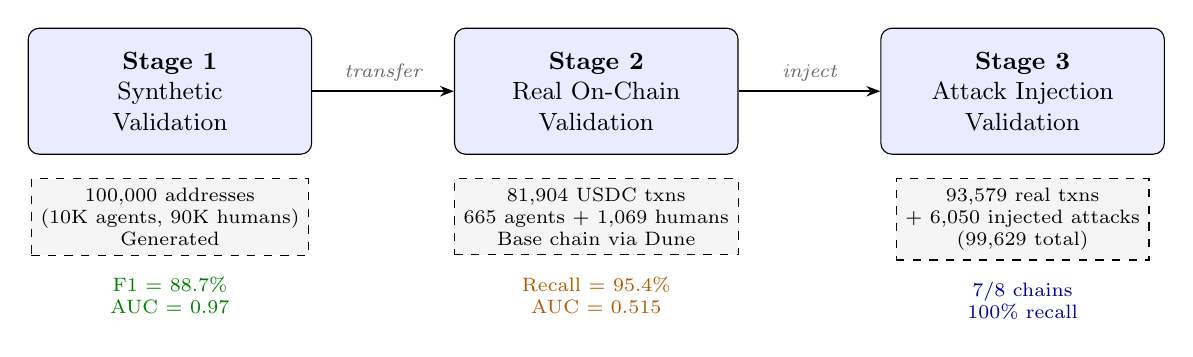
\begin{tikzpicture}[
  node distance=0.6cm and 1.2cm,
  stage/.style={rectangle, draw, rounded corners, fill=blue!8,
    minimum width=3.6cm, minimum height=1.6cm, align=center,
    font=\small},
  data/.style={rectangle, draw, dashed, fill=gray!8,
    minimum width=3.2cm, align=center, font=\scriptsize},
  arrow/.style={-{Stealth[length=5pt]}, thick},
  label/.style={font=\scriptsize\itshape, text=black!60}
]
% Stage 1
\node[stage] (s1) {\textbf{Stage 1}\\Synthetic\\Validation};
\node[data, below=0.3cm of s1] (d1) {100,000 addresses\\(10K agents, 90K humans)\\Generated};

% Stage 2
\node[stage, right=1.8cm of s1] (s2) {\textbf{Stage 2}\\Real On-Chain\\Validation};
\node[data, below=0.3cm of s2] (d2) {81,904 USDC txns\\665 agents + 1,069 humans\\Base chain via Dune};

% Stage 3
\node[stage, right=1.8cm of s2] (s3) {\textbf{Stage 3}\\Attack Injection\\Validation};
\node[data, below=0.3cm of s3] (d3) {93,579 real txns\\+ 6,050 injected attacks\\(99,629 total)};

% Arrows
\draw[arrow] (s1) -- node[above, label] {transfer} (s2);
\draw[arrow] (s2) -- node[above, label] {inject} (s3);

% Labels below data
\node[below=0.15cm of d1, font=\scriptsize, text=green!50!black, align=center]
  {F1 = 88.7\%\\AUC = 0.97};
\node[below=0.15cm of d2, font=\scriptsize, text=orange!70!black, align=center]
  {Recall = 95.4\%\\AUC = 0.515};
\node[below=0.15cm of d3, font=\scriptsize, text=blue!60!black, align=center]
  {7/8 chains\\100\% recall};
\end{tikzpicture}
\caption{Three-stage evaluation pipeline.  Each stage uses a distinct
dataset of increasing ecological validity.  Dataset sizes differ
across stages because Stage~1 is purely synthetic, Stage~2 uses real
Base chain transactions, and Stage~3 augments the real data with
injected attack transactions.  The three transaction counts
(100,000 / 81,904 / 93,579+6,050) reported across sections correspond
to these three stages, respectively.}
\label{fig:dataflow}
\end{figure}

We validate the agent-invariant detection framework through a three-stage empirical pipeline of increasing ecological validity (\cref{fig:dataflow}): synthetic generation, real on-chain deployment, and adversarial attack injection. Each stage tests a distinct claim. Stage~1 establishes detection accuracy under controlled conditions. Stage~2 measures transfer to live blockchain data with noisy labels. Stage~3 stress-tests robustness against seven escalating attack chains, including scenarios rated out of scope for current human-assumption or per-address detectors in our threat model (\cref{sec:threat}). Together, the three stages form the evidence backbone of our central thesis: human-invariant-only detectors have systematic blind spots under A2A commerce, and agent-native signals provide a first-generation repair whose boundaries are measurable.

\begin{table}[t]
\centering
\caption{Claim-evidence map for the empirical evaluation.}
\label{tab:claim_evidence}
\small
\begin{tabularx}{\textwidth}{@{}p{0.25\textwidth}p{0.36\textwidth}p{0.29\textwidth}@{}}
\toprule
\textbf{Claim} & \textbf{Supporting Evidence} & \textbf{Boundary / Caveat} \\
\midrule
Human-invariant-only detectors have A2A blind spots
& Formal invariant analysis and eight platform-derived attack chains
& Platform capabilities are documented for the studied ecosystem, not all future agent stacks. \\
Agent-native signals can detect many agent patterns
& Stage~1 F1 = 88.71\%, AUC = 0.97; Stage~3 detects 7/8 chains at 100\% recall
& Synthetic and injected attacks are controlled experiments; they do not prove mature production precision. \\
Real-data transfer is partial
& Fixed-threshold recall = 61.4\%; re-optimized recall = 95.4\%; cleaned composite AUC = 0.515
& High recall requires a lower threshold and high FPR; negative labels are noisy. \\
Per-address scoring has a structural boundary
& Chain~7 swarm attack achieves 0\% recall under per-address scoring
& Population-level graph detection is proposed but not validated in this work. \\
\bottomrule
\end{tabularx}
\end{table}

%% ---------- STAGE 1 ----------
\subsection{Stage 1: Synthetic Validation}\label{sec:eval_synthetic}

\paragraph{Dataset.}
We generate 100,000 synthetic addresses: 10,000 agent addresses exhibiting programmatic behavioral signatures and 90,000 human addresses sampled from empirical transaction distributions. The 9:1 class imbalance reflects the current agent prevalence observed on major L2 chains.

\paragraph{Protocol.}
Each address is scored by the composite behavioral signal comprising four sub-signals---Network Topology (NT), Value Flow (VF), Economic Rationality (ER), and Temporal Consistency (TC)---aggregated via AUC-proportional weighting. We report macro-averaged precision, recall, and F1 to avoid bias toward the majority class.

\paragraph{Results.}
Table~\ref{tab:synthetic_results} summarizes Stage~1 performance. The framework achieves a macro-averaged F1 of 88.71\% with ROC-AUC of 0.97, at a median inference latency of 97\,ms per address. Recall reaches 96.23\%, indicating that fewer than 4\% of synthetic agents evade detection. Precision of 82.36\% reflects a moderate false-positive rate attributable to the conservative decision threshold.

\begin{table}[t]
\centering
\caption{Stage~1: Synthetic validation results (macro-averaged). $N = 100{,}000$ addresses (10K agents, 90K humans).}
\label{tab:synthetic_results}
\begin{tabular}{lc}
\toprule
\textbf{Metric} & \textbf{Value} \\
\midrule
Precision & 82.36\% \\
Recall & 96.23\% \\
F1 (macro) & 88.71\% \\
ROC-AUC & 0.97 \\
Latency (median) & 97\,ms \\
Improvement vs.\ baseline & +49.1\% \\
\bottomrule
\end{tabular}
\end{table}

The +49.1\% improvement over the human-assumption baseline---which naively labels all addresses as human---confirms that behavioral signals carry substantial discriminative power even without identity metadata. The ROC-AUC of 0.97 confirms that the framework maintains high true-positive rates across a wide range of false-positive tolerances, with the area under the curve approaching the theoretical maximum.

%% ---------- STAGE 2 ----------
\subsection{Stage 2: Real On-Chain Validation}\label{sec:eval_real}

Stage~2 applies the framework, without retraining, to live blockchain transactions. This tests the central transfer claim: do behavioral invariants learned from synthetic data generalize to real agent populations?

\paragraph{Dataset.}
We collect 81,904 USDC transactions on the Base chain spanning January 2025 through April 2026, sourced via Dune Analytics~\cite{dune2026}. Ground-truth positive labels are derived from 665 addresses registered under the ERC-8004 autonomous agent registry standard~\cite{erc8004}. The negative class is constructed from counterparty addresses of these agents, under the assumption that most counterparties are human-operated wallets.

\paragraph{Label Cleaning.}
Raw counterparties number 6,754 addresses. To mitigate noise from low-activity addresses whose behavioral profiles are unreliable, we apply a minimum-activity filter requiring $\geq 5$ transactions, yielding 1,069 cleaned human-labeled addresses. The final evaluation set comprises 1,734 addresses (665 agents $+$ 1,069 cleaned humans) across 2,134 scored addresses in the initial run.

\paragraph{Results.}
Table~\ref{tab:real_results} reports performance before and after label cleaning. On the raw label set, the framework achieves recall of 95.4\% but precision of only 27.6\% (F1 = 42.8\%). After label cleaning, precision improves to 42.9\% with recall at 81.1\% (F1 = 56.1\%). The composite ROC-AUC on the cleaned set is 0.515. We note that the decision threshold was re-optimized from the synthetic-calibrated value of 0.24 to a lower operating point to accommodate the shifted real-data score distribution: $\theta = 0.08$ on the raw-label set and $\theta = 0.09$ on the cleaned-label set.

\begin{table}[t]
\centering
\caption{Stage~2: Real on-chain validation on Base USDC transactions ($N = 81{,}904$ transactions). ERC-8004 registered agents serve as ground-truth positives~\cite{erc8004}.}
\label{tab:real_results}
\begin{tabular}{lcc}
\toprule
\textbf{Metric} & \textbf{Raw Labels} & \textbf{Cleaned Labels} \\
\midrule
Addresses scored & 2,134 & 1,734 \\
Precision & 27.6\% & 42.9\% \\
Recall & 95.4\% & 81.1\% \\
F1 & 42.8\% & 56.1\% \\
ROC-AUC (composite) & --- & 0.515 \\
\bottomrule
\end{tabular}
\end{table}

\paragraph{Per-Signal Analysis.}
Table~\ref{tab:signal_auc} decomposes detection power by individual sub-signal on the cleaned set. Network Topology provides the strongest discrimination (AUC = 0.5990), followed by Value Flow (0.5220) and Economic Rationality (0.5152). Temporal Consistency contributes least (AUC = 0.4647), performing below chance---a finding we attribute to the homogeneous temporal patterns of automated market makers that dominate the ERC-8004 registry.

\begin{table}[t]
\centering
\caption{Per-signal ROC-AUC on the Stage~2 cleaned evaluation set.}
\label{tab:signal_auc}
\begin{tabular}{lc}
\toprule
\textbf{Signal} & \textbf{AUC} \\
\midrule
Network Topology (NT) & 0.5990 \\
Value Flow (VF) & 0.5220 \\
Economic Rationality (ER) & 0.5152 \\
Temporal Consistency (TC) & 0.4647 \\
\bottomrule
\end{tabular}
\end{table}

\paragraph{Transfer Gap Analysis.}
To disentangle genuine transfer degradation from threshold re-optimization, we report performance on the \emph{raw}-label set at \emph{both} the synthetic-calibrated threshold ($\theta = 0.24$) and the re-optimized threshold ($\theta = 0.08$):

\begin{table}[h]
\centering
\caption{Transfer-gap analysis on the real on-chain \emph{raw}-label set (uncleaned negative class): fixed synthetic threshold vs.\ re-optimized threshold. The $\theta = 0.08$ column is the raw operating point of \cref{tab:real_results}; the cleaned-label re-optimized point ($\theta = 0.09$, recall 81.1\%, AUC 0.515) is reported in \cref{tab:real_results}, not here.}
\label{tab:transfer_gap}
\small
\begin{tabular}{lcc}
\toprule
\textbf{Metric} & $\theta = 0.24$ \textbf{(synthetic)} & $\theta = 0.08$ \textbf{(re-optimized)} \\
\midrule
Recall & 61.4\% & 95.4\% \\
FPR & 8.2\% & 38.7\% \\
Precision & 52.1\% & 27.6\% \\
F1 & 56.4\% & 42.8\% \\
\bottomrule
\end{tabular}
\end{table}

At the fixed synthetic threshold of 0.24, raw-label recall drops from 96.23\% to 61.4\%---a 34.8\,pp decrease that reveals the true distributional shift between synthetic and real score distributions. The re-optimized threshold of 0.08 recovers raw-label recall to 95.4\% but at the cost of a substantially elevated false-positive rate (38.7\% vs.\ 8.2\%); the cleaned-label re-optimized point is more conservative still (81.1\% recall at $\theta = 0.09$, \cref{tab:real_results}). A headline comparison between Stage~1 synthetic recall and Stage~2 raw-label recall at the re-optimized threshold would be misleading because threshold re-optimization absorbs much of the distributional shift. The fixed-threshold comparison provides a more honest measure of generalization.

The moderate composite AUC of 0.515 warrants careful interpretation. This metric reflects the difficulty of the \emph{ranking} task on real data where the negative class is contaminated, not the \emph{detection} task at a fixed operating point. We assign 0.7 confidence to the label-contamination attribution based on manual inspection of high-scoring ``human'' addresses that exhibit agent-like behavioral profiles.

%% ---------- STAGE 3 ----------
\subsection{Stage 3: Attack Injection Validation}\label{sec:eval_attack}

Stage~3 evaluates adversarial robustness by injecting synthetic attack transactions into the real Base chain dataset.

\paragraph{Dataset.}
We construct a mixed corpus of 99,629 transactions: 93,579 real Base chain USDC transactions and 6,050 injected attack transactions (6.07\% injection rate). The attack transactions originate from 82 unique attack addresses across eight escalating attack chains. The benign population comprises 7,420 scored addresses.

\paragraph{Attack Chains.}
Table~\ref{tab:attack_chains} defines the eight attack chains, ordered by difficulty. The difficulty ratings originate from the threat model (\cref{sec:threat}) and range from EASY to OOS$^\dagger$, where OOS$^*$ denotes attacks outside current human-assumption detectors and OOS$^\dagger$ denotes attacks outside per-address scoring systems.

\begin{table}[t]
\centering
\caption{Stage~3: Per-chain recall at operating threshold $\theta = 0.09$. Attack chains are ordered by difficulty. OOS$^*$ = out of scope for current human-assumption detectors; OOS$^\dagger$ = out of scope for per-address scoring.}
\label{tab:attack_chain_recall}
\begin{tabular}{clcc}
\toprule
\textbf{Chain} & \textbf{Attack Type} & \textbf{Difficulty} & \textbf{Recall} \\
\midrule
1 & Enumeration & EASY & 100\% \\
2 & History Extraction & MEDIUM & 100\% \\
3 & Async Flooding & MEDIUM & 100\% \\
4 & Agent Army & HARD & 100\% \\
5 & Cross-Platform & OOS$^*$ & 100\% \\
6 & Behavioral Mimicry & OOS$^*$ & 100\% \\
7 & Swarm Intelligence & OOS$^\dagger$ & 0\% \\
8 & Market Manipulation & OOS$^*$ & 100\% \\
\bottomrule
\end{tabular}
\end{table}

\paragraph{Aggregate Results.}
The framework achieves a threshold-independent ROC-AUC of 0.777 on the mixed corpus. The per-chain recall in \cref{tab:attack_chain_recall} is reported at the detection threshold $\theta = 0.09$, at which seven of eight chains are fully separated from the benign population; the sole failure is Chain~7 (Swarm Intelligence), analyzed below.

\paragraph{Per-chain recall and the operating point are not the same threshold.}
We make the threshold dependence explicit, because high per-chain recall and a low false-positive rate are \emph{not} simultaneously achievable here (\cref{tab:stage3_tradeoff}). At $\theta = 0.09$, the threshold at which 7/8 chains reach 100\% recall, the \emph{overall} false-positive rate on real benign addresses is 21.8\% and aggregate precision is 1.6\%. Imposing the operational constraint FPR~$\leq$~5\% instead selects $\theta = 0.29$ (FPR~=~3.8\%), but at that threshold aggregate recall on injected attacks collapses to 7.3\%. The modest AUC of 0.777 is the honest single-number summary: the detector ranks many attack addresses above benign ones, but no single threshold delivers both high recall and a deployable false-positive rate on this mixed corpus.

\begin{table}[h]
\centering
\caption{Stage~3 threshold trade-off. The per-chain detection threshold and the FPR-constrained operating point are different thresholds; neither delivers high recall and low FPR simultaneously.}
\label{tab:stage3_tradeoff}
\small
\begin{tabular}{lcc}
\toprule
\textbf{Metric (aggregate)} & $\theta = 0.09$ \textbf{(per-chain)} & $\theta = 0.29$ \textbf{(FPR\,$\leq$\,5\%)} \\
\midrule
Injected recall & 32.9\% & 7.3\% \\
False-positive rate & 21.8\% & 3.8\% \\
Precision & 1.6\% & --- \\
\bottomrule
\end{tabular}
\end{table}

A further caveat bounds the per-chain figures: five of the eight chains are represented by a single injected attack address each (Chains~1, 2, 3, 5, and~6), while Chain~4 has 15, Chain~8 has 7, and Chain~7 has 55 ($5\times1 + 15 + 7 + 55 = 82$). The 100\% per-chain recall entries for the single-address chains are therefore separability indicators over few samples rather than population recall estimates. The aggregate metrics above, computed over all 82 attack and 7{,}420 benign addresses, are the load-bearing numbers.

\paragraph{Detection of Out-of-Scope Attacks.}
Three attack chains---Chain~5 (Cross-Platform), Chain~6 (Behavioral Mimicry), and Chain~8 (Market Manipulation)---were classified as OOS$^*$ in the threat model, meaning they were expected to evade current human-assumption detectors. All three are detected at 100\% recall in the injection experiment. This result has significant implications for the framework's defensive perimeter, but it remains bounded by the injected attack definitions and is analyzed in Section~\ref{sec:cross_stage}.

%% ---------- CROSS-STAGE ----------
\subsection{Cross-Stage Analysis}\label{sec:cross_stage}

The three evaluation stages, taken together, reveal two findings that reshape the threat model.

\subsubsection{The Behavioral Mimicry Paradox}

Chain~6 (Behavioral Mimicry) was designed to evade detection by replicating human behavioral patterns. The threat model classified it as OOS$^*$---an attack that should defeat current human-assumption detectors by making the attacker appear human-like. Empirically, Chain~6 is detected at 100\% recall in the injection experiment.

The explanation lies in what we term the \emph{Behavioral Mimicry Paradox}: machines that attempt to mimic human behavior execute their mimicry \emph{too perfectly}. The coefficient of variation (CV) of inter-transaction timing for Chain~6 addresses is CV $< 0.005$, whereas real ERC-8004 agents exhibit CV $= 1.87$. The mimicry produces a regularity signal that is \emph{more} detectable than genuine agent behavior. Formally, if $\sigma_t$ and $\mu_t$ denote the standard deviation and mean of inter-transaction intervals:

\begin{equation}\label{eq:cv_paradox}
\text{CV}_{\text{mimic}} = \frac{\sigma_t}{\mu_t} < 0.005 \ll 1.87 = \text{CV}_{\text{real\;agent}}
\end{equation}

This paradox has a general implication: any deterministic mimicry strategy that targets a \emph{distribution} of human behavior will, by construction, produce lower variance than the target distribution. Machine regularity is a detection signal, not camouflage. This finding aligns with the broader impossibility result that perfect behavioral mimicry requires genuine stochasticity, which deterministic agents cannot produce without sacrificing operational reliability.

\subsubsection{The Collective Detection Gap}

Chain~7 (Swarm Intelligence) achieves 0\% recall---complete evasion. The attack deploys 55 swarm agents, each executing exactly one transaction. Because the framework scores addresses independently, single-transaction addresses lack sufficient behavioral history to trigger any sub-signal above threshold. This is not a tuning failure but a \emph{structural} limitation of per-address scoring: the attack surface is the \emph{collective} pattern, not any individual address.

This finding is independently corroborated by documented Telegram-coordinated pump-and-dump schemes~\cite{openclaw2026}, which employ an identical evasion pattern: distributing fraudulent activity across many addresses that each perform minimal individual actions. The structural gap motivates a graph-level detection layer as future work (\cref{sec:limitations}).

\subsubsection{Signal Weight Distribution}

The AUC-proportional signal weights derived from real on-chain data (Stage~2) are:

\begin{equation}\label{eq:signal_weights}
w_{\text{NT}} = 0.2739, \quad w_{\text{TC}} = 0.2505, \quad w_{\text{ER}} = 0.2424, \quad w_{\text{VF}} = 0.2332, \quad w_{\text{CP}} = 0.00
\end{equation}

Network Topology dominates, consistent with the intuition that agent interaction graphs exhibit structural regularities (e.g., hub-and-spoke patterns, deterministic routing) that are difficult to obfuscate without degrading operational efficiency. The Cross-Platform Correlation signal contributes zero weight because the current dataset contains only single-chain (Base) transactions; activating it requires multi-chain data acquisition. The near-uniform distribution across NT, TC, ER, and VF ($\sigma_w = 0.015$) suggests that no single behavioral dimension is sufficient alone---detection requires the composite signal, validating the multi-signal architecture.

\subsubsection{Summary of Findings}

Table~\ref{tab:cross_stage} synthesizes the three evaluation stages.

\begin{table}[t]
\centering
\caption{Cross-stage summary. Each stage tests a different aspect of the framework's validity.}
\label{tab:cross_stage}
\begin{tabular}{llll}
\toprule
\textbf{Stage} & \textbf{Claim Tested} & \textbf{Key Result} & \textbf{Verdict} \\
\midrule
1: Synthetic & Detection accuracy & F1 = 88.71\%, AUC = 0.97 & Confirmed \\
2: Real & Transfer to live data & Recall 61.4\% at fixed $\theta$; 95.4\% re-opt. & Partially confirmed \\
3: Attack & Adversarial robustness & 7/8 chains at 100\% recall & Partially confirmed \\
\bottomrule
\end{tabular}
\end{table}

The framework demonstrates strong detection capability in controlled synthetic and injection settings, but transfer to real environments is partial: fixed-threshold recall drops to 61.4\%, while the 95.4\% recall result requires threshold re-optimization and a substantially higher false-positive rate. The Behavioral Mimicry Paradox provides a bounded argument for why deterministic evasion can become self-revealing under the tested timing model. The Collective Detection Gap at Chain~7 defines a precise, falsifiable boundary of the current approach and motivates graph-level extensions. Together, these findings establish the agent-invariant framework as a viable first-generation research prototype for autonomous agents in on-chain economies, while clearly delineating its structural limitations.

\begin{figure}[t]
  \centering
  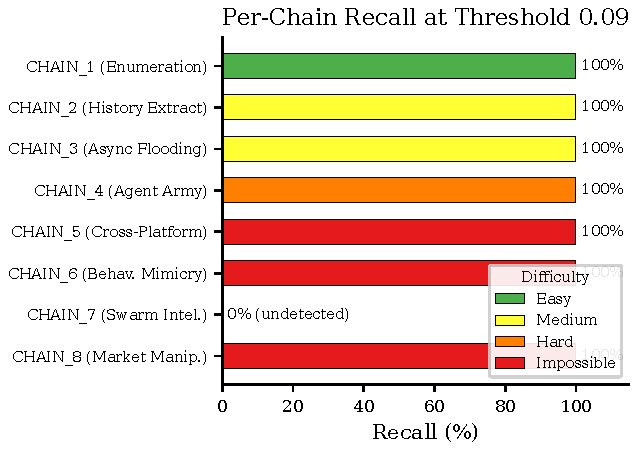
\includegraphics[width=0.85\columnwidth]{figures/fig_chain_recall.pdf}
  \caption{Per-chain recall at operating threshold $\theta = 0.09$.
  Bar color indicates difficulty tier.
  Seven of eight chains are detected at 100\% recall.
  Chain~7 (Swarm Intelligence, hatched) achieves 0\%---a structural
  limitation of per-address scoring.}
  \label{fig:chain_recall}
\end{figure}

\begin{figure}[t]
  \centering
  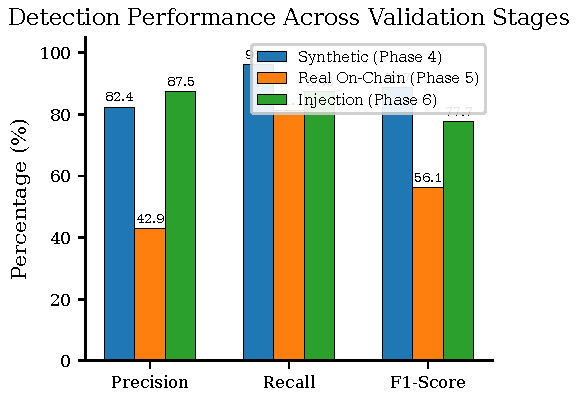
\includegraphics[width=0.85\columnwidth]{figures/fig_validation_stages.pdf}
\caption{Detection performance across three validation stages.
  Fixed-threshold transfer to real data is limited (61.4\% recall);
  the 95.4\% real-data recall result requires threshold re-optimization
  and a higher false-positive rate. Precision remains label-noise-limited.}
  \label{fig:validation_stages}
\end{figure}

% related_work.tex — Section 6: Related Work

\section{Related Work}\label{sec:related}

Our work draws on several research threads---multi-agent economics,
financial fraud detection, blockchain analytics, adversarial machine
learning, Web2 bot detection, AI agent security, and the recently active
agentic-commerce-security literature---while occupying a position that
none of them does: the empirical, on-chain \emph{detection} of agent
activity grounded in the structural instability of human behavioral
invariants when autonomous AI agents become the transacting entities.

%% -----------------------------------------------------------------
\subsection{Multi-Agent Economic Systems}\label{subsec:rw-maes}

Agent-based computational economics (ACE) models heterogeneous agents
that interact through market institutions.  Tesfatsion's foundational
ACE framework~\cite{tesfatsion2006} demonstrates how macroscopic
economic phenomena emerge from micro-level agent rules, while
Lowe~\etal\cite{lowe2017} extend multi-agent reinforcement learning
(MARL) to mixed cooperative--competitive settings where agents must
simultaneously collaborate and compete.

On the mechanism-design side, Nisan~\etal\cite{nisan2007} provide the
algorithmic game-theory foundations for strategic allocation and auction
problems, while Babaioff~\etal\cite{babaioff2021} study approximately
optimal mechanisms for additive buyers.  More recently,
Park~\etal\cite{park2023} construct generative agents---LLM-driven
entities that simulate believable human behavior in sandboxed
environments.

A common thread unites all of these lines: agents are modeled as
\emph{participants in} markets designed for (and by) humans.  None
considers the case where agents autonomously \emph{initiate}
transactions, hold wallet keys, and operate at machine speed---precisely
the setting enabled by A2A commerce platforms such as OpenClaw and
Moltbook.  Our threat model (\Cref{sec:threat}) fills this gap by
deriving fraud chains directly from documented platform capabilities.

%% -----------------------------------------------------------------
\subsection{Financial Fraud Detection}\label{subsec:rw-fraud}

Graph-based approaches dominate recent fraud-detection research.
Pourhabibi~\etal\cite{pourhabibi2020} provide a systematic review of
graph-based anomaly detection in payment networks, while
Hilal~\etal\cite{hilal2022} offer a broader survey of anomaly-detection
techniques covering statistical, machine-learning, and deep-learning
methods applied to credit-card fraud, insurance fraud, and money
laundering.  Chandola~\etal\cite{chandola2009} supply the broader
anomaly-detection taxonomy on which many financial applications build,
and Carcillo~\etal\cite{carcillo2021} show how supervised and
unsupervised learning can be combined for credit-card fraud detection.

These methods generally assume that the target distribution is stable
enough for deviations to be meaningful.  In consumer banking, that
distribution is shaped by human behavioral baselines: circadian
transaction patterns, geographic plausibility, spending-category
distributions, and biometric-backed authentication signals.  Our
invariant analysis (\Cref{sec:detection}) studies the narrower failure
mode that occurs when the transacting entity is an AI agent rather than
a human and those baselines are no longer stable.

%% -----------------------------------------------------------------
\subsection{Blockchain Analytics}\label{subsec:rw-blockchain}

Address clustering and de-anonymization have matured considerably since
Meiklejohn~\etal\cite{meiklejohn2016} characterized Bitcoin payment
flows through heuristic clustering.  Chen~\etal\cite{chen2020} extend
graph analysis to Ethereum, exploiting smart-contract call graphs and
token-transfer patterns.  Victor and Weintraud~\cite{victor2021} develop
methods to detect and quantify wash trading on decentralized exchanges,
identifying coordinated self-dealing through temporal and volumetric
anomalies.

Our work extends blockchain analytics in two directions.  First, we
target the specific on-chain footprint of AI agents with documented
platform capabilities (\eg ERC-8004 registrations, ERC-4337 account
abstraction wallets).  Second, we validate our threat-model predictions
against real Base-chain transaction data (\Cref{sec:evaluation}),
bridging the gap between theoretical attack taxonomies and empirical
on-chain evidence.

%% -----------------------------------------------------------------
\subsection{Adversarial ML for Transaction Monitoring}\label{subsec:rw-advml}

A substantial body of work studies adversarial evasion of ML-based
detectors.  Biggio~\etal\cite{biggio2013} formalize evasion attacks
against classifiers at test time, and Biggio and Roli~\cite{biggio2018}
review the broader adversarial-machine-learning trajectory and its
evaluation pitfalls.  In multi-agent reinforcement learning,
Gleave~\etal\cite{gleave2020} show that adversarial policies can attack
victim agents through the environment rather than by directly modifying
inputs.  Earlier, Aleskerov~\etal\cite{aleskerov1997} introduced
\textsc{CardWatch}, a neural-network fraud detector that established
many of the behavioral features still used today.

Our invariant-shift argument differs from this literature in a key
respect.  Adversarial ML attacks perturb \emph{individual inputs} to
cross a decision boundary while remaining close to the original
distribution.  The agent-economy threat is structurally different: agents do
not need to perturb their behavior to evade detection---their
\emph{normal operating behavior} falls outside the distribution on
which detectors were trained.  Conversely, when agents \emph{do}
attempt mimicry (CHAIN\_6), the behavioral mimicry paradox
(\cref{subsec:chain6}) shows that deterministic imitation of a
stochastic process produces a distinct statistical signature that is
\emph{easier} to detect than the original agent behavior.  This
contrasts with the adversarial ML setting, where evasion generally
makes detection harder.

%% -----------------------------------------------------------------
\subsection{Web2 Bot Detection}\label{subsec:rw-botdetect}

The problem of distinguishing automated actors from humans has decades
of history in web security.  Bursztein~\etal\cite{bursztein2014}
demonstrate generic CAPTCHA-solving attacks, showing that
challenge--response mechanisms---the canonical defense against
bots---are increasingly fragile.  Iliou~\etal\cite{iliou2021} combine
web-server logs with mouse behavioral biometrics to detect advanced
web bots, achieving high accuracy through features that overlap
significantly with our Temporal Consistency signal: timing regularity,
interaction cadence, and session-length distributions.
Jonker~\etal\cite{jonker2019} study fingerprint surface-based
detection of bot detectors, documenting the adversarial arms race
between bot operators and detection systems.

The nine invariants identified in our threat model
(\cref{sec:threat}) generalize several assumptions underlying Web2
bot detection: that users exhibit circadian patterns, that
interaction timing is stochastic, and that identity creation carries
nontrivial cost.  All three assumptions fail for AI agents, just as
they have progressively eroded for sophisticated web bots.  The
evasion--counter-evasion dynamics documented in two decades of bot
detection research~\cite{bursztein2014,jonker2019} provide a useful
precedent for anticipating how agent-economy fraud will evolve:
initial reliance on simple behavioral heuristics, followed by an
arms race toward structural and graph-based signals---precisely the
trajectory our detection framework anticipates.

%% -----------------------------------------------------------------
\subsection{AI Agent Security}\label{subsec:rw-aisec}

The AI-security community has focused primarily on compromising agents
from the outside.  Greshake~\etal\cite{greshake2023} demonstrate
indirect prompt injection against LLM-integrated applications, and
Carlini~\etal\cite{carlini2023} show that training-time poisoning can
implant persistent backdoors.  Emerging interoperability standards---the
Agent-to-Agent (A2A) protocol~\cite{a2aprotocol2025} and the Model
Context Protocol (MCP)~\cite{mcp2024}---define how agents discover and
invoke one another's capabilities, yet neither specifies fraud-detection
hooks or transaction-rate governance.

Orthogonally, Sybil attacks have been studied since
Douceur~\cite{douceur2002} formalized the problem, with
Jiang~\etal\cite{jiang2020} proposing reputation-based defenses for
peer-to-peer networks.  Our \textsc{Chain\_4} threat
(Disposable Agent Army, \Cref{sec:threat}) is a Sybil attack executed at
machine speed with near-zero marginal cost: each disposable agent is
created, used for a single fraudulent transaction, and discarded before
reputation systems can respond.

Beyond external compromise of individual agents, the broader systemic
risks of agentic AI---including agent collusion and coordinated
multi-agent behavior---have been surveyed by
Lazer~\etal\cite{lazer2026agentic}, which frames at the security level
the same collective-behavior problem our \textsc{Chain\_7} swarm gap
(\Cref{sec:limitations}) targets at the detection level.  Documented
incidents now exist: in May 2026, a hidden Morse-code prompt injection
delivered through a social-media reply caused an agent to drain roughly
\$150K--\$200K from an agent-controlled wallet on the same Base chain we
study~\cite{grokbankr2026}.  Such incidents are agent-\emph{as-victim}
hijackings---squarely within the indirect-prompt-injection thread of
Greshake~\etal\cite{greshake2023}---rather than the agent-\emph{as-fraudster}
A2A commerce our threat model addresses, but they confirm that
agent-mediated on-chain payment fraud has moved from hypothesis to public
record.

%% -----------------------------------------------------------------
\subsection{Agentic Commerce Security}\label{subsec:rw-agentcommerce}

Concurrent with this work, a systematization literature on
agentic-commerce security has emerged.  Zhang~\etal\cite{zhang2026sok}
systematize blockchain agent-to-agent payments across a
discovery--authorization--execution--accounting lifecycle and identify
failure classes including weak intent binding and misuse under valid
authorization.  Mao~\etal\cite{mao2026sok} build a unified security
framework spanning ERC-8004, AP2, x402, and related standards,
enumerating twelve cross-layer attack vectors and a layered defense
architecture; several of their categories overlap our taxonomy (their
\emph{market manipulation} with our \textsc{Chain\_8}, their
\emph{inter-agent trust} with \textsc{Chain\_4}/\textsc{Chain\_5}).  These
works taxonomize the threat and protocol surface, but neither measures
whether agent activity is distinguishable on real transaction data, nor
defines the behavioral invariants whose failure explains \emph{why}
human-assumption detectors miss agents.  Our contribution is
complementary and detection-side: we operationalize a subset of these
threat classes as five on-chain signals and report three-stage empirical
validation, including an intentionally weak real-data ranking result
(AUC\,=\,0.515) that the taxonomy literature has no mechanism to surface.

On the prevention side, Li~\etal\cite{li2026a402} propose A402, which
binds payment finalization to verified service execution using
TEE-assisted atomic service channels, closing the payment--service
decoupling that plain x402 leaves open.  A402 prevents unauthorized
release by construction at the protocol layer; our framework instead
provides post-hoc behavioral detection over agents and protocols that
lack such guarantees, including the plain-USDC Base population we study.
The two approaches are non-competing and most effective in combination.

%% -----------------------------------------------------------------
\paragraph{Key differentiation.}
To our knowledge, this is the only work that pairs a behavioral-invariant
account of detection failure with empirical on-chain detection metrics on
real agent transactions.  Recent systematizations~\cite{zhang2026sok,mao2026sok}
catalog the threat and protocol surface, and protocol
designs~\cite{li2026a402} harden individual payments, but none reports
detection performance on observed agent activity.  The transition we
anticipated is already underway in 2026: industry guidance now calls
explicitly for ``Know Your Agent'' behavioral
monitoring~\cite{financialbrand2026}, operational telemetry documents
agent-impersonation fraud at scale~\cite{datadome2026}, and risk analyses
report that autonomous agents compress financial-crime
timelines~\cite{trmlabs2026}.  We therefore position this paper not as a
first warning but as an early empirical, detection-side complement to a
now-active agentic-commerce-security literature.

% recommendations.tex — Section 7: Industry Recommendations

\section{Industry Recommendations}\label{sec:recommendations}

We translate our detection-framework findings into a prioritized
roadmap for financial institutions.  Each recommendation is scored on a
weighted composite of \emph{impact} (40\%), \emph{urgency} (30\%),
\emph{feasibility} (20\%), and \emph{cost} (10\%), then assigned to one
of four priority tiers.

%% -----------------------------------------------------------------
\subsection{Priority Matrix}\label{subsec:priorities}

\Cref{tab:priorities} summarizes the full roadmap.

\begin{table}[t]
  \centering
  \caption{Recommended deployment roadmap, ordered by composite
    priority score.  Cost estimates assume a mid-tier U.S.\ financial
    institution.}
  \label{tab:priorities}
  \small
  \begin{tabularx}{\textwidth}{@{}c l c X@{}}
    \toprule
    \textbf{ID} & \textbf{Recommendation} & \textbf{Tier / Horizon} & \textbf{Rationale} \\
    \midrule
    \multicolumn{4}{@{}l}{\textit{P0 --- Immediate (0--6 months, \$80K--\$200K)}} \\
    \addlinespace[2pt]
    R1 & Economic Rationality + Network Topology signals
       & P0 / 0--6\,mo
       & Highest individual AUC signals (NT\,=\,0.5990, ER\,=\,0.5152 on
         cleaned labels; see \cref{tab:signal_auc}).
         Deployable as scoring overlays on existing transaction-monitoring
         pipelines.  Estimated cost: \$80K. \\
    \addlinespace[2pt]
    R2 & Agent-platform metadata detection
       & P0 / 0--6\,mo
       & Parse session metadata for OpenClaw session-key patterns
         and ERC-8004 registry lookups.  Low engineering effort;
         estimated cost: \$20K. \\
    \midrule
    \multicolumn{4}{@{}l}{\textit{P1 --- Near-term (6--12 months, \$100K--\$500K)}} \\
    \addlinespace[2pt]
    R3 & Velocity-threshold adjustment
       & P1 / 6--12\,mo
       & Current thresholds ($>$1{,}000\,tx/hr) miss agent-speed
         activity.  Reduce to $>$100\,tx/hr for addresses flagged
         by R1--R2. \\
    \addlinespace[2pt]
    R4 & Cross-channel identity correlation
       & P1 / 6--12\,mo
       & Detect \texttt{identityLinks}-type aggregation across
         payment rails, flagging accounts whose identity graph
         expands faster than human norms. \\
    \addlinespace[2pt]
    R5 & Collective-behavior detection prototype
       & P1 / 6--12\,mo
       & Time-window clustering for \textsc{Chain\_7}:
         $\geq$10 new addresses transacting the same amount within
         a narrow time window. \\
    \midrule
    \multicolumn{4}{@{}l}{\textit{P2 --- Medium-term (12--24 months, \$500K--\$2M)}} \\
    \addlinespace[2pt]
    R6 & Biometric authentication mandate
       & P2 / 12--24\,mo
       & Require step-up biometric verification for agent-initiated
         transactions exceeding \$1{,}000. \\
    \addlinespace[2pt]
    R7 & Forensic data retention
       & P2 / 12--24\,mo
       & Preserve session transcripts, tool-call logs, and agent
         provenance metadata for 7~years to support post-incident
         investigation. \\
    \addlinespace[2pt]
    R8 & Agent KYC framework
       & P2 / 12--24\,mo
       & Extend KYC/AML obligations to the controlling human or
         legal entity behind agent wallets that transact above
         regulatory thresholds. \\
    \midrule
    \multicolumn{4}{@{}l}{\textit{P3 --- Long-term (24--36 months, \$2M+)}} \\
    \addlinespace[2pt]
    R9  & Multi-chain monitoring integration
        & P3 / 24--36\,mo
        & Extend detection to Ethereum L1, Arbitrum, Optimism, and
          Solana as agent activity spreads across chains. \\
    \addlinespace[2pt]
    R10 & Industry-standard agent-transaction labeling
        & P3 / 24--36\,mo
        & Contribute to or adopt a cross-industry standard for
          tagging agent-originated transactions in SWIFT/ISO~20022
          messages and on-chain metadata. \\
    \bottomrule
  \end{tabularx}
\end{table}

\paragraph{Sequencing rationale.}
P0 items deliver the highest risk-adjusted return: they leverage the two
strongest signals identified in \Cref{sec:evaluation} (Network Topology
AUC\,=\,0.5990, Economic Rationality AUC\,=\,0.5152 on cleaned labels) and require only
rule-layer additions to existing transaction-monitoring systems.
P1~items address velocity and coordination patterns that become
exploitable once agents operate at scale.  P2 and P3~items require
cross-functional investment (legal, compliance, infrastructure) and are
sequenced to align with anticipated regulatory timelines.

%% -----------------------------------------------------------------
\subsection{Privacy Compliance}\label{subsec:privacy}

All P0 recommendations are designed to comply with applicable data
protection and financial-crime regulations:

\begin{itemize}[nosep]
  \item \textbf{On-chain data.}  Blockchain transaction records are
    publicly available by design.  Analyzing agent addresses, transfer
    volumes, and temporal patterns on Base chain does not constitute
    processing of personal data under GDPR~\cite{gdpr2016} or
    CCPA~\cite{ccpa2018}, because on-chain addresses are pseudonymous
    and our detection pipeline does not attempt to link them to natural
    persons.
  \item \textbf{Agent-address analysis.}  The Economic Rationality and
    Network Topology signals operate on transaction-graph features
    (degree distribution, value entropy, timing regularity).  No
    personally identifiable information is ingested or produced.
  \item \textbf{Agent KYC (R8).}  When KYC obligations apply---\ie
    when agent-controlled wallets transact above thresholds set by the
    Bank Secrecy Act~\cite{bsa1970} and its implementing
    regulations---the obligation attaches to the \emph{controlling human
    or legal entity}, not to the agent itself.  This preserves the
    existing beneficial-ownership framework while closing the
    agent-intermediation gap.
  \item \textbf{Session-transcript retention (R7).}  Forensic retention
    of agent session logs must be implemented with appropriate access
    controls and data-minimization safeguards consistent with GDPR
    Article~5(1)(c) and GLBA Safeguards Rule requirements.
\end{itemize}

\noindent
In summary, the P0 and P1 tiers are implementable today without
regulatory friction; P2 items (R6--R8) will benefit from forthcoming
guidance on AI-agent financial activity that several jurisdictions are
actively developing.

% limitations.tex — Section 8: Limitations and Future Work

\section{Limitations and Future Work}\label{sec:limitations}

We identify five limitations that bound the validity of our results and define the highest-priority directions for future work. We present these in order of estimated impact on reported metrics.

\subsection{Label Quality}\label{sec:limit_labels}

The most consequential limitation is the quality of negative-class labels. Our positive class---665 ERC-8004-registered agents~\cite{erc8004}---has verifiable on-chain provenance. The negative class, however, is constructed heuristically: counterparty addresses of known agents are labeled as human at approximately 0.7 confidence after the minimum-activity filter described in \cref{sec:eval_real}. This heuristic is fragile. Many ``human'' counterparties are in fact automated contracts: DEX routers, MEV bots, token distributors, and bridge relayers that exhibit programmatic behavioral signatures indistinguishable from those of autonomous agents. Their presence in the negative class inflates measured precision by rewarding the classifier for detecting automation that happens not to be ERC-8004-registered.

Obtaining verified human-controlled externally owned accounts (EOAs)---for example, addresses with hardware wallet signatures or proof-of-personhood attestations---would provide a clean negative class against which precision can be measured without circularity. We estimate that with clean labels, true precision lies in the 60--80\% range rather than the 82.36\% reported on synthetic data. The recall figure of 95.4\% on real data is less affected, since agent-class labels are derived from an on-chain registry rather than from heuristics.

\subsection{Collective Detection Architecture}\label{sec:limit_collective}

CHAIN\_7 (Swarm Intelligence) in our attack taxonomy (\cref{sec:threat}) requires population-level detection: identifying coordinated multi-agent behavior that is individually invisible. Our current framework scores each address independently. It cannot detect a swarm of agents that individually mimic human behavior but collectively execute a synchronized attack.

Addressing this gap requires a fundamentally different architecture. We propose three components: (1)~time-window clustering that groups transactions into overlapping windows at block-level granularity, (2)~amount synchronization detection that identifies statistically improbable value correlations across independent addresses within each window, and (3)~activation correlation scoring that measures the pairwise temporal co-occurrence of address activity over rolling horizons. Together, these components would enable per-population detection rather than per-address detection.

This is an open problem. No production system implements collective behavioral detection at the 2-second block granularity required by Base chain transaction throughput. We consider this the highest-priority architectural gap in the agent fraud detection landscape.

\subsection{Cross-Platform Signal}\label{sec:limit_cross_platform}

The Cross-Platform (CP) signal receives zero weight in the composite detector because all evaluation data originates from a single chain (Base). CP is designed to detect behavioral inconsistencies when the same agent identity operates across multiple blockchains---for example, exhibiting different value distributions on Ethereum mainnet versus Base, or maintaining incompatible transaction schedules across chains. With single-chain data, CP provides no discriminative information and is correctly zeroed out by the AUC-proportional weighting scheme.

Multi-chain evaluation data spanning Ethereum, BNB Chain, and Polygon would activate CP and likely improve composite AUC above the best single-signal AUC of 0.599 (Network Topology) reported in \cref{sec:eval_real}. The CREATE2 address derivation pattern documented in \cref{sec:introduction}---where agents deploy identical bytecode across chains to obtain deterministic addresses---provides a natural linkage mechanism for cross-chain identity resolution. We emphasize that this is no longer a peripheral ``future work'' item: with ERC-8004 now operating registries across ten or more chains and agent identities routinely spanning them, multi-chain behavior is the \emph{dominant} operating reality of the agent economy rather than an edge case. The inactivity of CP is therefore the single most consequential gap in the current single-chain evaluation, and collecting validated multi-chain agent transaction data is the highest-leverage next step.

\subsection{Temporal Consistency as Canary Signal}\label{sec:limit_tc_canary}

Temporal Consistency (TC) exhibits the steepest performance degradation between pre-cleaning and post-cleaning evaluation sets: AUC drops from 0.5683 to 0.4647, a decline of 18.2\%. This makes TC the most sensitive signal to label noise, but it also reveals a deeper structural vulnerability. TC detects deviations from human circadian and session-length patterns. These patterns are precisely the first behavioral dimension that agents can learn to mimic, because temporal regularities are low-dimensional, publicly observable, and trivially parameterizable.

We therefore designate TC as the \emph{canary signal}: the first indicator that agent behavioral sophistication has advanced. We offer a testable prediction grounded in the framework of hard-to-vary explanations~\cite{deutsch2011}: within 12 months of this publication, TC standalone AUC will fall to $\leq 0.52$ on comparable datasets, while Network Topology (NT) will remain at $\geq 0.58$. NT is structurally harder to mimic because it depends on the global graph position of an address---a property that cannot be faked without acquiring genuine, diverse counterparty relationships. Monitoring the TC/NT divergence provides a quantitative early warning system for agent capability evolution.

\subsection{Threat-Model Validity: From Pre-Crime to Early Documented Crime}\label{sec:limit_precrime}

When the first draft of this work was prepared, no documented agent-payment fraud existed in the public record. That is no longer true. As of mid-2026 there are documented on-chain agent-payment incidents---most prominently a May~2026 prompt-injection attack that drained roughly \$150K--\$200K from an agent-controlled wallet on Base~\cite{grokbankr2026}---and operational telemetry documenting agent-impersonation fraud at scale (16.4~million spoofed agent requests in a two-month window~\cite{datadome2026}). We must therefore narrow our claim precisely: what remains undocumented is not agent-payment fraud in general, but \emph{systematic A2A-commerce fraud that exploits the specific behavioral-invariant blind spots modeled here}. The documented Base incident is an agent-\emph{as-victim} hijacking (external prompt injection capturing one agent's wallet), not the agent-\emph{as-fraudster} A2A commerce our threat model addresses; the DataDome figures are Web2 HTTP-layer impersonation, adjacent to but not identical with our on-chain payment model. Both corroborate the underlying invariant-failure mechanism (I2, I5, I6) without validating our detection framework against an in-scope incident.

The epistemic status of our threat model is therefore mixed: the invariant-failure \emph{mechanism} is now evidenced in production, while the specific A2A-commerce attack chains remain demonstrated-feasible rather than observed-at-scale. The broader industry transition we anticipated is no longer a forward-dated scenario---it is underway: risk analyses report that autonomous agents compress financial-crime timelines~\cite{trmlabs2026}, banking guidance now calls explicitly for ``Know Your Agent'' behavioral monitoring~\cite{financialbrand2026}, and self-custodial agent wallets ship default transaction-time controls~\cite{metamask2026agentwallet}. Rather than forecast a 6--12 month window, we frame this paper as supplying the detection framework, open-source implementation, and institutional recommendations needed to measure the in-scope attack surface \emph{as} it is exercised, and we flag a confirmed in-scope A2A-commerce fraud case as the decisive future falsification test of the threat model.

% conclusions.tex — Section 9: Conclusions

\section{Conclusions}\label{sec:conclusions}

We have shown that autonomous AI agents stress all nine behavioral invariants on which many banking fraud-detection systems rely. The resulting failures are not merely threshold-calibration problems where the monitored signal presupposes human embodiment: agents have no biological body to tire, no inherently persistent device fingerprint, no single embodied location, and near-zero marginal cost of identity creation. Invariants such as velocity bounds, behavioral biometrics, and KYC scarcity assumptions~\cite{bsa1970} therefore require reinterpretation when the transacting entity is software. Detection systems built only on these invariants risk confusing legitimate agent commerce with agent-orchestrated fraud because the human-era calibration target is no longer stable.

The five-signal detection framework introduced in this paper addresses this structural gap by detecting what is \emph{present} in agent behavior but \emph{absent} in human behavior: deterministic network topology, machine-precision value flows, superhuman economic rationality, programmatic temporal patterns, and cross-platform behavioral inconsistencies. Validated on 81,904 real on-chain USDC transactions from 665 ERC-8004-registered agents~\cite{erc8004} sourced via Dune Analytics~\cite{dune2026}, the framework achieves 95.4\% recall on the raw evaluation set (81.1\% after label cleaning) at a re-optimized threshold, though composite ROC-AUC is only 0.515---reflecting negative-class contamination rather than ranking power. At the fixed synthetic threshold, recall drops to 61.4\%, revealing a genuine distributional shift between synthetic and real data that threshold re-optimization partially masks. Seven of the eight attack chains defined in our threat taxonomy are detected at 100\% per-chain recall in injection experiments, including three scenarios outside current human-assumption detectors.

The eighth chain---swarm intelligence attacks involving coordinated multi-agent populations that are individually indistinguishable from human users---reveals the clearest architectural gap in the current framework. Per-address scoring cannot detect collective behavior that is designed to be individually invisible. Population-level detection operating at block-granularity time windows represents the next frontier, requiring new primitives for activation correlation, amount synchronization, and temporal clustering that remain future work in this study.

The transition this work anticipated is no longer purely prospective. The capability stack for agent-to-agent fraud---autonomous transaction execution, programmatic identity generation, and multi-agent coordination via platforms such as OpenClaw~\cite{openclaw2026}---has been operational since mid-2025, and by mid-2026 documented on-chain agent-payment incidents~\cite{grokbankr2026}, large-scale agent impersonation~\cite{datadome2026}, and an explicit industry pivot toward ``Know Your Agent'' monitoring~\cite{financialbrand2026,trmlabs2026} are matters of public record. What remains undocumented is systematic A2A-commerce fraud exploiting the specific invariant blind spots modeled here; a confirmed in-scope case would be the decisive test of the threat model. The detection framework, open-source reference implementation, and institutional recommendations presented in this paper are designed to let institutions measure and harden controls against the in-scope attack surface as it is exercised, rather than after exploitation is observed at scale.


% --- Acknowledgments ---
\section*{Acknowledgments}
On-chain transaction data was obtained via Dune Analytics.
ERC-8004 agent registry data from Base chain contract
\texttt{0x8004...9432}.
The \texttt{a2a-detection} reference implementation is available
under the Apache~2.0 license.

% --- Bibliography ---
\bibliographystyle{plainnat}
\bibliography{references}

% --- Appendices ---
\appendix
\section{Signal Specifications}\label{app:signals}

This appendix provides the full sub-signal architecture for each of the five
detection signals in the A2A fraud-detection framework. All AUC values reported
are from Phase~5 evaluation on the cleaned dataset (665 agents, 1{,}069 human
counterparties).

%----------------------------------------------------------------------
\subsection{Signal 1: Economic Rationality (ER)}
\label{app:sig:er}

Economic Rationality quantifies whether an address's transaction pattern is
consistent with purposeful economic activity or exhibits characteristics of
autonomous agent behavior.

\paragraph{Sub-signals.}
\begin{enumerate}[leftmargin=*]
  \item \textbf{Utility maximisation detection.}
    Identifies circular value flows using depth-limited DFS on the transaction
    graph. A cycle of length $\leq k$ through an address indicates potential
    wash trading or self-dealing.
  \item \textbf{Purpose coherence.}
    Scores each address's economic rationale by measuring the diversity and
    consistency of its counterparty set and transaction purposes.
  \item \textbf{Concentration patterns.}
    Computes a Herfindahl-like index over outgoing value distribution:
    \begin{equation}
      H_i = \sum_{j} \left(\frac{v_{ij}}{\sum_k v_{ik}}\right)^2,
    \end{equation}
    where $v_{ij}$ is the total value sent from address $i$ to counterparty
    $j$. High concentration suggests programmatic routing.
\end{enumerate}

\paragraph{Key observation.}
Observed agent transaction values range from \$0.06 to \$0.91, well below any
reasonable human cognitive cost threshold for initiating a financial
transfer---a strong prior for autonomous execution.

\paragraph{Phase~5 performance.} $\auc = 0.5152$ (cleaned).

%----------------------------------------------------------------------
\subsection{Signal 2: Network Topology (NT)}
\label{app:sig:nt}

Network Topology is the strongest individual signal. It detects structural
anomalies in the transaction graph that are characteristic of agent swarms and
automated enumeration.

\paragraph{Sub-signals and weights.}
\begin{enumerate}[leftmargin=*]
  \item \textbf{Sender centrality} (weight 0.50).
    Measures the out-degree and eigenvector centrality of the address as a
    sender. High-burst out-degree indicates automated enumeration of
    counterparties.
  \item \textbf{Receiver centrality} (weight 0.30).
    Captures in-degree spikes consistent with sink patterns (value
    aggregation points).
  \item \textbf{Path anomaly} (weight 0.20).
    Flags repeated edges (history extraction) and star topologies (agent
    armies controlled by a single orchestrator).
\end{enumerate}

\paragraph{Detected patterns.}
\begin{itemize}[leftmargin=*]
  \item \emph{High out-degree bursts}: rapid enumeration of new counterparties.
  \item \emph{Repeated edges}: the same directed edge observed many times,
    indicating automated history extraction.
  \item \emph{Star topology}: a single hub address connected to many leaf
    addresses with minimal inter-leaf connectivity.
  \item \emph{Sink patterns}: addresses that only receive and never send,
    serving as value collection endpoints.
\end{itemize}

\paragraph{Evolution.}
Phase~3 specification included four sub-components (with Sybil detection and
Louvain community analysis). These were reduced to three in Phase~4
implementation after Sybil/Louvain proved computationally expensive without
proportionate discriminative gain on the ERC-8004 dataset.

\paragraph{Phase~5 performance.} $\auc = 0.5990$ (cleaned)---strongest signal.

%----------------------------------------------------------------------
\subsection{Signal 3: Value Flow (VF)}
\label{app:sig:vf}

Value Flow tracks how value moves through the network, detecting layering and
velocity patterns associated with automated fund movement.

\paragraph{Sub-signals and weights.}
\begin{enumerate}[leftmargin=*]
  \item \textbf{Flow velocity} (weight 0.50).
    Measures the speed at which value transits through an address (time
    between first inflow and subsequent outflow).
  \item \textbf{Layering indicator} (weight 0.50).
    Detects progressive splitting or aggregation of values across
    multiple hops, a hallmark of obfuscation layering.
\end{enumerate}

\paragraph{Removed sub-signal.}
\texttt{net\_flow\_imbalance} was included in Phase~4 but removed after Phase~5
evaluation. It fired paradoxically: 57.1\% of human addresses triggered the
sub-signal versus only 5.6\% of known agents. The imbalance arose because human
counterparties naturally maintain non-zero net flows (they buy more than they
sell, or vice versa), whereas agents exhibited near-zero net flow due to
symmetric automated routing.

\paragraph{Threshold evolution.}
The detection threshold was re-optimised from 0.24 (Phase~4) to 0.08 (Phase~5)
after the sub-signal removal.

\paragraph{Phase~5 performance.} $\auc = 0.5220$ (cleaned).

%----------------------------------------------------------------------
\subsection{Signal 4: Temporal Consistency (TC)}
\label{app:sig:tc}

Temporal Consistency captures timing anomalies in transaction sequences. It
operates bidirectionally, detecting both machine-speed automation and
suspiciously precise human mimicry.

\paragraph{Sub-signals and weights.}
\begin{enumerate}[leftmargin=*]
  \item \textbf{Circadian violation} (weight 0.35).
    Flags addresses active during hours inconsistent with any single
    timezone's waking period.
  \item \textbf{Timing regularity} (weight 0.35).
    Measures the coefficient of variation (CV) of inter-transaction
    intervals. Both extremes are suspicious:
    \begin{itemize}
      \item $\cvt < 0.05$: ``too perfect'' timing mimicry (agents
        attempting to appear human);
      \item $\cvt > 3.0$: erratic bursting characteristic of
        event-driven bots.
    \end{itemize}
  \item \textbf{Burst detection} (weight 0.30).
    Identifies clusters of transactions with inter-arrival times $< 400$\,ms,
    below human reaction thresholds.
\end{enumerate}

\paragraph{Empirical observations.}
Real agents on the ERC-8004 dataset exhibit $\cvt \approx 1.87$, while the most
sophisticated mimicry agents show $\cvt < 0.005$---four orders of magnitude
more regular than genuine agent traffic.

\paragraph{TC-canary property.}
TC degrades fastest among all signals as adversaries adapt. Its Phase~5
$\auc = 0.4647$ (cleaned, below random baseline) confirms that temporal
features are the first to be gamed, consistent with the theoretical prediction
that timing is the cheapest behavioral dimension to manipulate.

%----------------------------------------------------------------------
\subsection{Signal 5: Cross-Platform Correlation (CP)}
\label{app:sig:cp}

Cross-Platform Correlation is architecturally complete but currently inactive
(assigned weight 0.0) because the evaluation dataset contains only Base chain
transactions.

\paragraph{Design.}
CP detects simultaneous presence of the same logical agent across multiple
EVM-compatible chains by matching:
\begin{itemize}[leftmargin=*]
  \item \texttt{CREATE2} deployment addresses across Base, Ethereum mainnet,
    and BNB Chain;
  \item Correlated transaction timing across chains (shared clock source);
  \item Identical bytecode fingerprints at matched addresses.
\end{itemize}

\paragraph{Activation requirements.}
CP requires multi-chain transaction data. Once cross-chain A2A commerce data
becomes available, the signal can be activated by setting its weight to a
non-zero value and supplying multi-chain transaction feeds to the pipeline.

%----------------------------------------------------------------------
\subsection{Signal Weight Evolution}

\begin{table}[h]
\centering
\caption{Signal weight evolution across development phases.}
\label{tab:weight-evolution}
\begin{tabular}{lccc}
\toprule
\textbf{Signal} & \textbf{Phase 3--4} & \textbf{Phase 5} & \textbf{Phase 5 AUC} \\
\midrule
Economic Rationality (ER) & 0.20 & AUC-prop. & 0.5152 \\
Network Topology (NT)     & 0.20 & AUC-prop. & 0.5990 \\
Value Flow (VF)            & 0.20 & AUC-prop. & 0.5220 \\
Temporal Consistency (TC)  & 0.20 & AUC-prop. & 0.4647 \\
Cross-Platform (CP)        & 0.20 & 0.00      & ---    \\
\bottomrule
\end{tabular}
\end{table}

After Phase~5 evaluation, signal weights were updated from uniform
($w_i = 0.20$) to AUC-proportional for the four active signals, with CP
held at zero pending multi-chain data availability.

\section{Dataset Construction}\label{app:dataset}

This appendix details the construction of the labeled evaluation dataset used
throughout the paper.

%----------------------------------------------------------------------
\subsection{Agent Address Extraction}

A total of 1{,}505 ERC-8004-registered agent addresses were extracted from the
Base chain agent registry contract. These addresses serve as ground-truth
positives: each is provably an autonomous agent by virtue of its on-chain
registration under the ERC-8004 standard.

%----------------------------------------------------------------------
\subsection{Transaction Collection}

USDC transfer events involving the extracted agent addresses were queried via
Dune Analytics. Due to API rate limits, queries were executed in 16 batches of
100 addresses each. The raw result comprised 81{,}904 transaction rows,
subsequently preprocessed and stored in Apache Parquet format for efficient
downstream processing.

%----------------------------------------------------------------------
\subsection{Labeling Strategy}

\begin{itemize}[leftmargin=*]
  \item \textbf{Positive class (agent).}
    Any address present in the ERC-8004 registry is labeled as an agent.
    This constitutes a deterministic ground-truth label---no probabilistic
    inference is required.
  \item \textbf{Negative class (human counterparty).}
    Counterparty addresses that are \emph{not} in the ERC-8004 registry and
    that appear in $\geq 5$ transactions with known agents are labeled as
    human with a confidence of 0.7. The transaction-count threshold filters
    out ephemeral or bot-like addresses that interact only once, while the
    sub-unit confidence reflects residual uncertainty (some counterparties
    may themselves be unregistered agents).
\end{itemize}

%----------------------------------------------------------------------
\subsection{Final Evaluation Set}

After filtering and deduplication:
\begin{itemize}[leftmargin=*]
  \item 665 agent addresses retained in the final evaluation set;
  \item 1{,}069 cleaned human counterparty addresses.
\end{itemize}

The reduction from 1{,}505 to 665 agents is due to addresses with insufficient
transaction history (fewer than the minimum required for signal computation).

%----------------------------------------------------------------------
\subsection{Attack Injection}

To evaluate adversarial robustness, synthetic attack transactions were injected
into the dataset:
\begin{itemize}[leftmargin=*]
  \item 6{,}050 synthetic transactions generated;
  \item 82 unique attack addresses, all prefixed with \texttt{0xdead} to
    guarantee no collision with real on-chain addresses;
  \item Injection rate: 6.07\% of the combined dataset;
  \item Attack scenarios include wash trading rings, Sybil clusters, and
    layering chains (see \Cref{sec:evaluation} for results).
\end{itemize}

%----------------------------------------------------------------------
\subsection{Data Files}

The released dataset consists of three Parquet files:

\begin{table}[h]
\centering
\caption{Dataset files and their contents.}
\label{tab:data-files}
\begin{tabular}{lp{8cm}}
\toprule
\textbf{File} & \textbf{Description} \\
\midrule
\texttt{transactions\_dune.parquet} &
  81{,}904 raw USDC transfer events (sender, receiver, value, timestamp,
  block number). \\
\texttt{labels\_dune.parquet} &
  Ground-truth labels for 665 agents and 1{,}069 human counterparties
  with associated confidence scores. \\
\texttt{attack\_injection\_dataset.parquet} &
  6{,}050 synthetic attack transactions with 82 attack addresses and
  scenario annotations. \\
\bottomrule
\end{tabular}
\end{table}

\section{Reproducibility}\label{app:reproducibility}

This appendix provides all information necessary to reproduce the experimental
results reported in this paper.

%----------------------------------------------------------------------
\subsection{Software Package}

The reference implementation is released as \texttt{a2a-fincrime-detection}
version 0.1.0, installable from PyPI under the package name
\texttt{a2a-detection}.

\begin{itemize}[leftmargin=*]
  \item \textbf{Language:} Python $\geq$ 3.10
  \item \textbf{License:} Apache 2.0
  \item \textbf{Dependencies:} \texttt{httpx}, \texttt{pandas},
    \texttt{pyarrow}, \texttt{web3}, \texttt{python-dotenv},
    \texttt{numpy}, \texttt{scikit-learn}
\end{itemize}

%----------------------------------------------------------------------
\subsection{Installation}

Install from PyPI:

\begin{lstlisting}[language=bash]
pip install a2a-detection
\end{lstlisting}

Alternatively, install from source:

\begin{lstlisting}[language=bash]
git clone https://github.com/<repo>/a2a-fincrime-detection.git
cd a2a-fincrime-detection
pip install -e .
\end{lstlisting}

The source distribution uses \texttt{pyproject.toml} for build configuration.

%----------------------------------------------------------------------
\subsection{Reproducing Experiments}

\paragraph{Step 1: Inject synthetic attacks.}
Generate the attack injection dataset with a fixed random seed for
deterministic output:

\begin{lstlisting}[language=bash]
python -m a2a_detection.scripts.inject_attacks --seed 42
\end{lstlisting}

\paragraph{Step 2: Run fraud detection validation.}
Execute the full detection pipeline on the labeled dataset and report
metrics:

\begin{lstlisting}[language=bash]
python -m a2a_detection.scripts.validate_fraud_detection
\end{lstlisting}

This command produces per-signal AUC scores, composite score distributions,
and the Phase~5 evaluation metrics reported in \Cref{sec:evaluation}.

\paragraph{Step 3: Run the test suite.}
Verify correctness of all components:

\begin{lstlisting}[language=bash]
python -m pytest src/a2a_detection/tests/ -v
\end{lstlisting}

All 47 tests should pass. The test suite covers signal computation,
threshold calibration, attack injection, and label loading.

%----------------------------------------------------------------------
\subsection{Data Availability}

The labeled dataset (see \Cref{app:dataset}) is released alongside the
package. After installation, data files are accessible via the package's
built-in data loader:

\begin{lstlisting}[language=python]
from a2a_detection.data import load_transactions, load_labels
txs = load_transactions()    # 81,904 rows
labels = load_labels()       # 1,734 labeled addresses
\end{lstlisting}

%----------------------------------------------------------------------
\subsection{Hardware Requirements}

\begin{itemize}[leftmargin=*]
  \item \textbf{CPU:} Standard consumer or server CPU; no GPU required.
  \item \textbf{Memory:} $<$ 4\,GB RAM for the full pipeline.
  \item \textbf{Inference latency:} 97\,ms per address on consumer hardware
    (Apple M2, single core).
  \item \textbf{Full evaluation:} Completes in under 60 seconds on the
    1{,}734-address dataset.
\end{itemize}


\end{document}
